\chapter{空间电源系统脆弱性量化分析}
\label{cha:Test}
\section{引言}
\label{sec:chap5:int}
依据本文所建立的控制系统脆弱性分析方法,对空间电源系统元件参数不确定性进行脆弱性分析。根据所建立的脆弱性量化评估模型对电源系统关键元器件的不确定性建模并进行脆弱性量化评估,根据量化结果评估元件不确定性对系统脆弱程度的影响,识别空间电源系统薄弱环节,为空间电源系统电路设计、系统集成以及参数优化提供理论依据。

本章以基于~Buck~变换器的空间电源系统为例,分别对~Buck~变换器主拓扑电路中电容元件、电感元件以及电阻元件的不确定性进行脆弱性量化评估,明确系统脆弱性量化评估的方法与具体步骤。对于量化评估结果进行分析,得到基于~Buck~变换器的空间电源系统脆弱性分析结果与系统薄弱环节。

\section{空间电源系统数学模型}
\label{sec:chap5:condition}
\subsection{基于~Buck~变换器空间电源系统的工作原理}
\label{sub:chap5:environment}
空间电源控制系统~(Power Conditioning Unit, PCU)~主要负责卫星在轨运行时整个能源的调节和分配,典型的空间电源控制系统主要由分流模块、充电模块~(BCR)~和放电模块~(BDR)~组成,分流模块主要采用顺序开关分流调节~(Sequential Switching Shunt Regulator,S3R)~架构\cite{Xin2007S3R,Rouzies2015Analysis,Guo2010SpacePower,Wang2012Development}。根据太阳能电池阵供电电流大小,调节空间电源控制系统工作在分流模块、充电模块或放电模块,从而维持母线电压的稳定。

鉴于空间电源控制系统结构过于复杂,且具体电路拓扑及元件参数属于保密范畴,因此本文选择空间电源控制系统中放电模块~(BDR)~的核心简化电源系统~\raisebox{0.5mm}{------}~基于~Buck~变换器的电源系统作为研究对象,进行脆弱性分析与量化评估。

选择文献~\cite{BuckXu}~中经过参数矫正后的基于~Buck~变换器的电源系统作为研究对象,电源系统模型图以及电路拓扑图分别如图~\ref{fig:chap5:powermodel}~与~\ref{fig:chap5:powertopology}~所示。图中,输入电压与输出电压分别为~$V_{g}$~和~$V_{out}$,~Buck~变换器主拓扑由滤波电感~L~、滤波电容~C~、续流二极管~VD~以及场效应管(MOSFET)~ S~组成。输出端分压反馈信号经过补偿环节得到的~PWM~波信号~d~来控制场效应管的开关,通过设计补偿网络的电阻与电容参数,优化电源系统的性能参数。

电路分析软件~Saber~仿真得到的电源系统频率响应~Bode~图以及~Nyquist~图分别如图~\ref{fig:chap5:bodegraph}~与图~\ref{fig:chap5:nyquist}~所示,经过补偿环节矫正的系统幅频特性在~20~kHz~处以~-20~dB/dec~斜率穿越~0dB~线,相位裕度经矫正后从之前的~$8.6^\circ$~提高到较为理想的~$66^\circ$~,改善了电源系统的幅值与相位裕度。

\begin{figure}[h]
  \centering
  % Requires \usepackage{graphicx}
     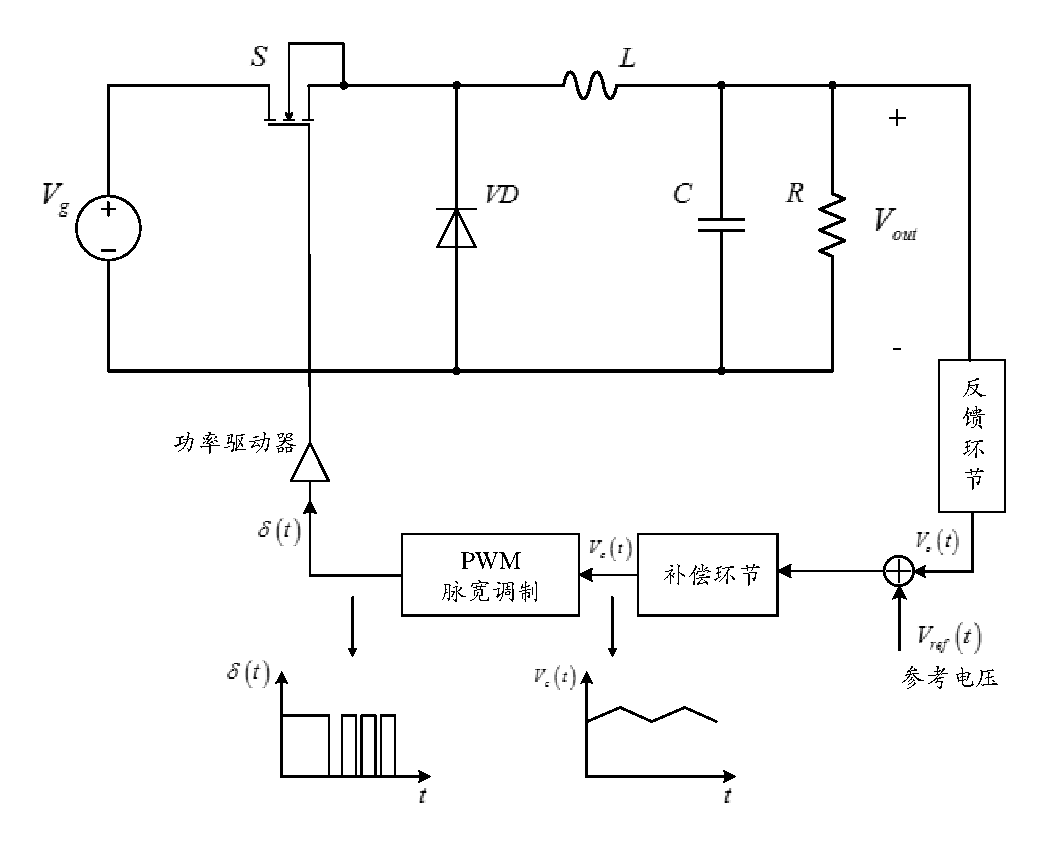
\includegraphics[width=11cm]{PowerModel.pdf}\\
  %\includegraphics[width=12cm]{test_speed_step.png}\\
  \caption{基于~Buck~变换器空间电源系统模型}\label{fig:chap5:powermodel}
\end{figure}

\begin{figure}[h]
  \centering
  % Requires \usepackage{graphicx}
     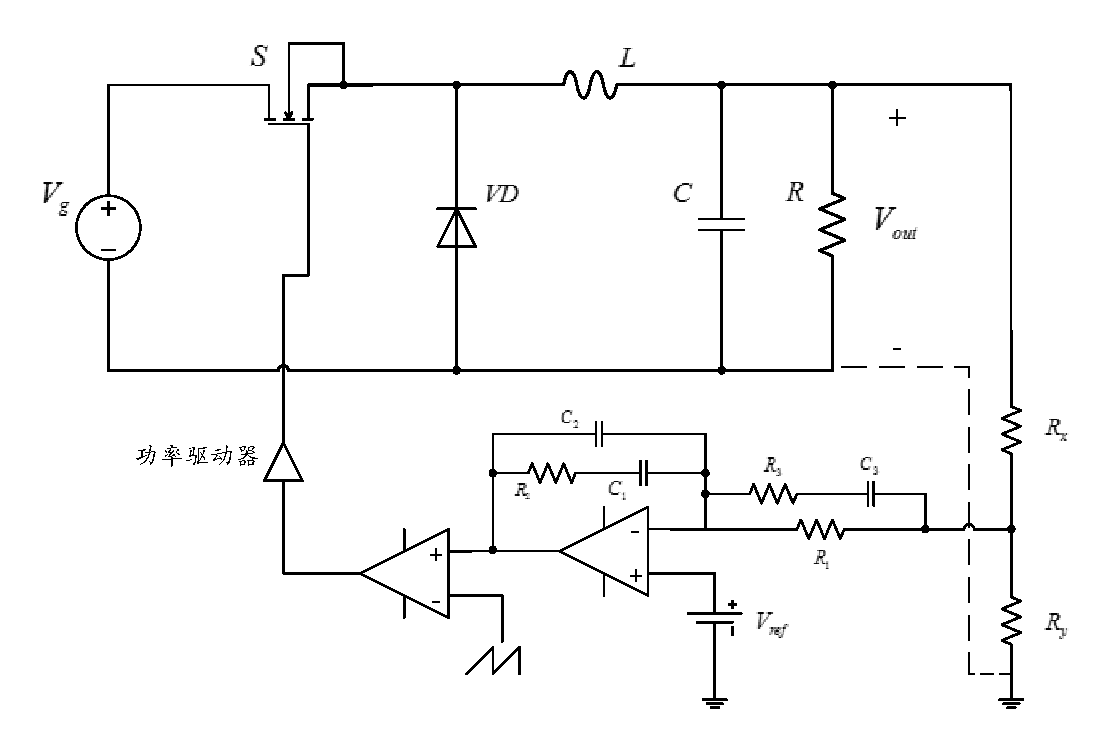
\includegraphics[width=11cm]{PowerTopology.pdf}\\
  %\includegraphics[width=12cm]{test_speed_step.png}\\
  \caption{基于~Buck~变换器空间电源系统拓扑图}\label{fig:chap5:powertopology}
\end{figure}
\iffalse
\begin{figure}[h]
  \centering
  % Requires \usepackage{graphicx}
     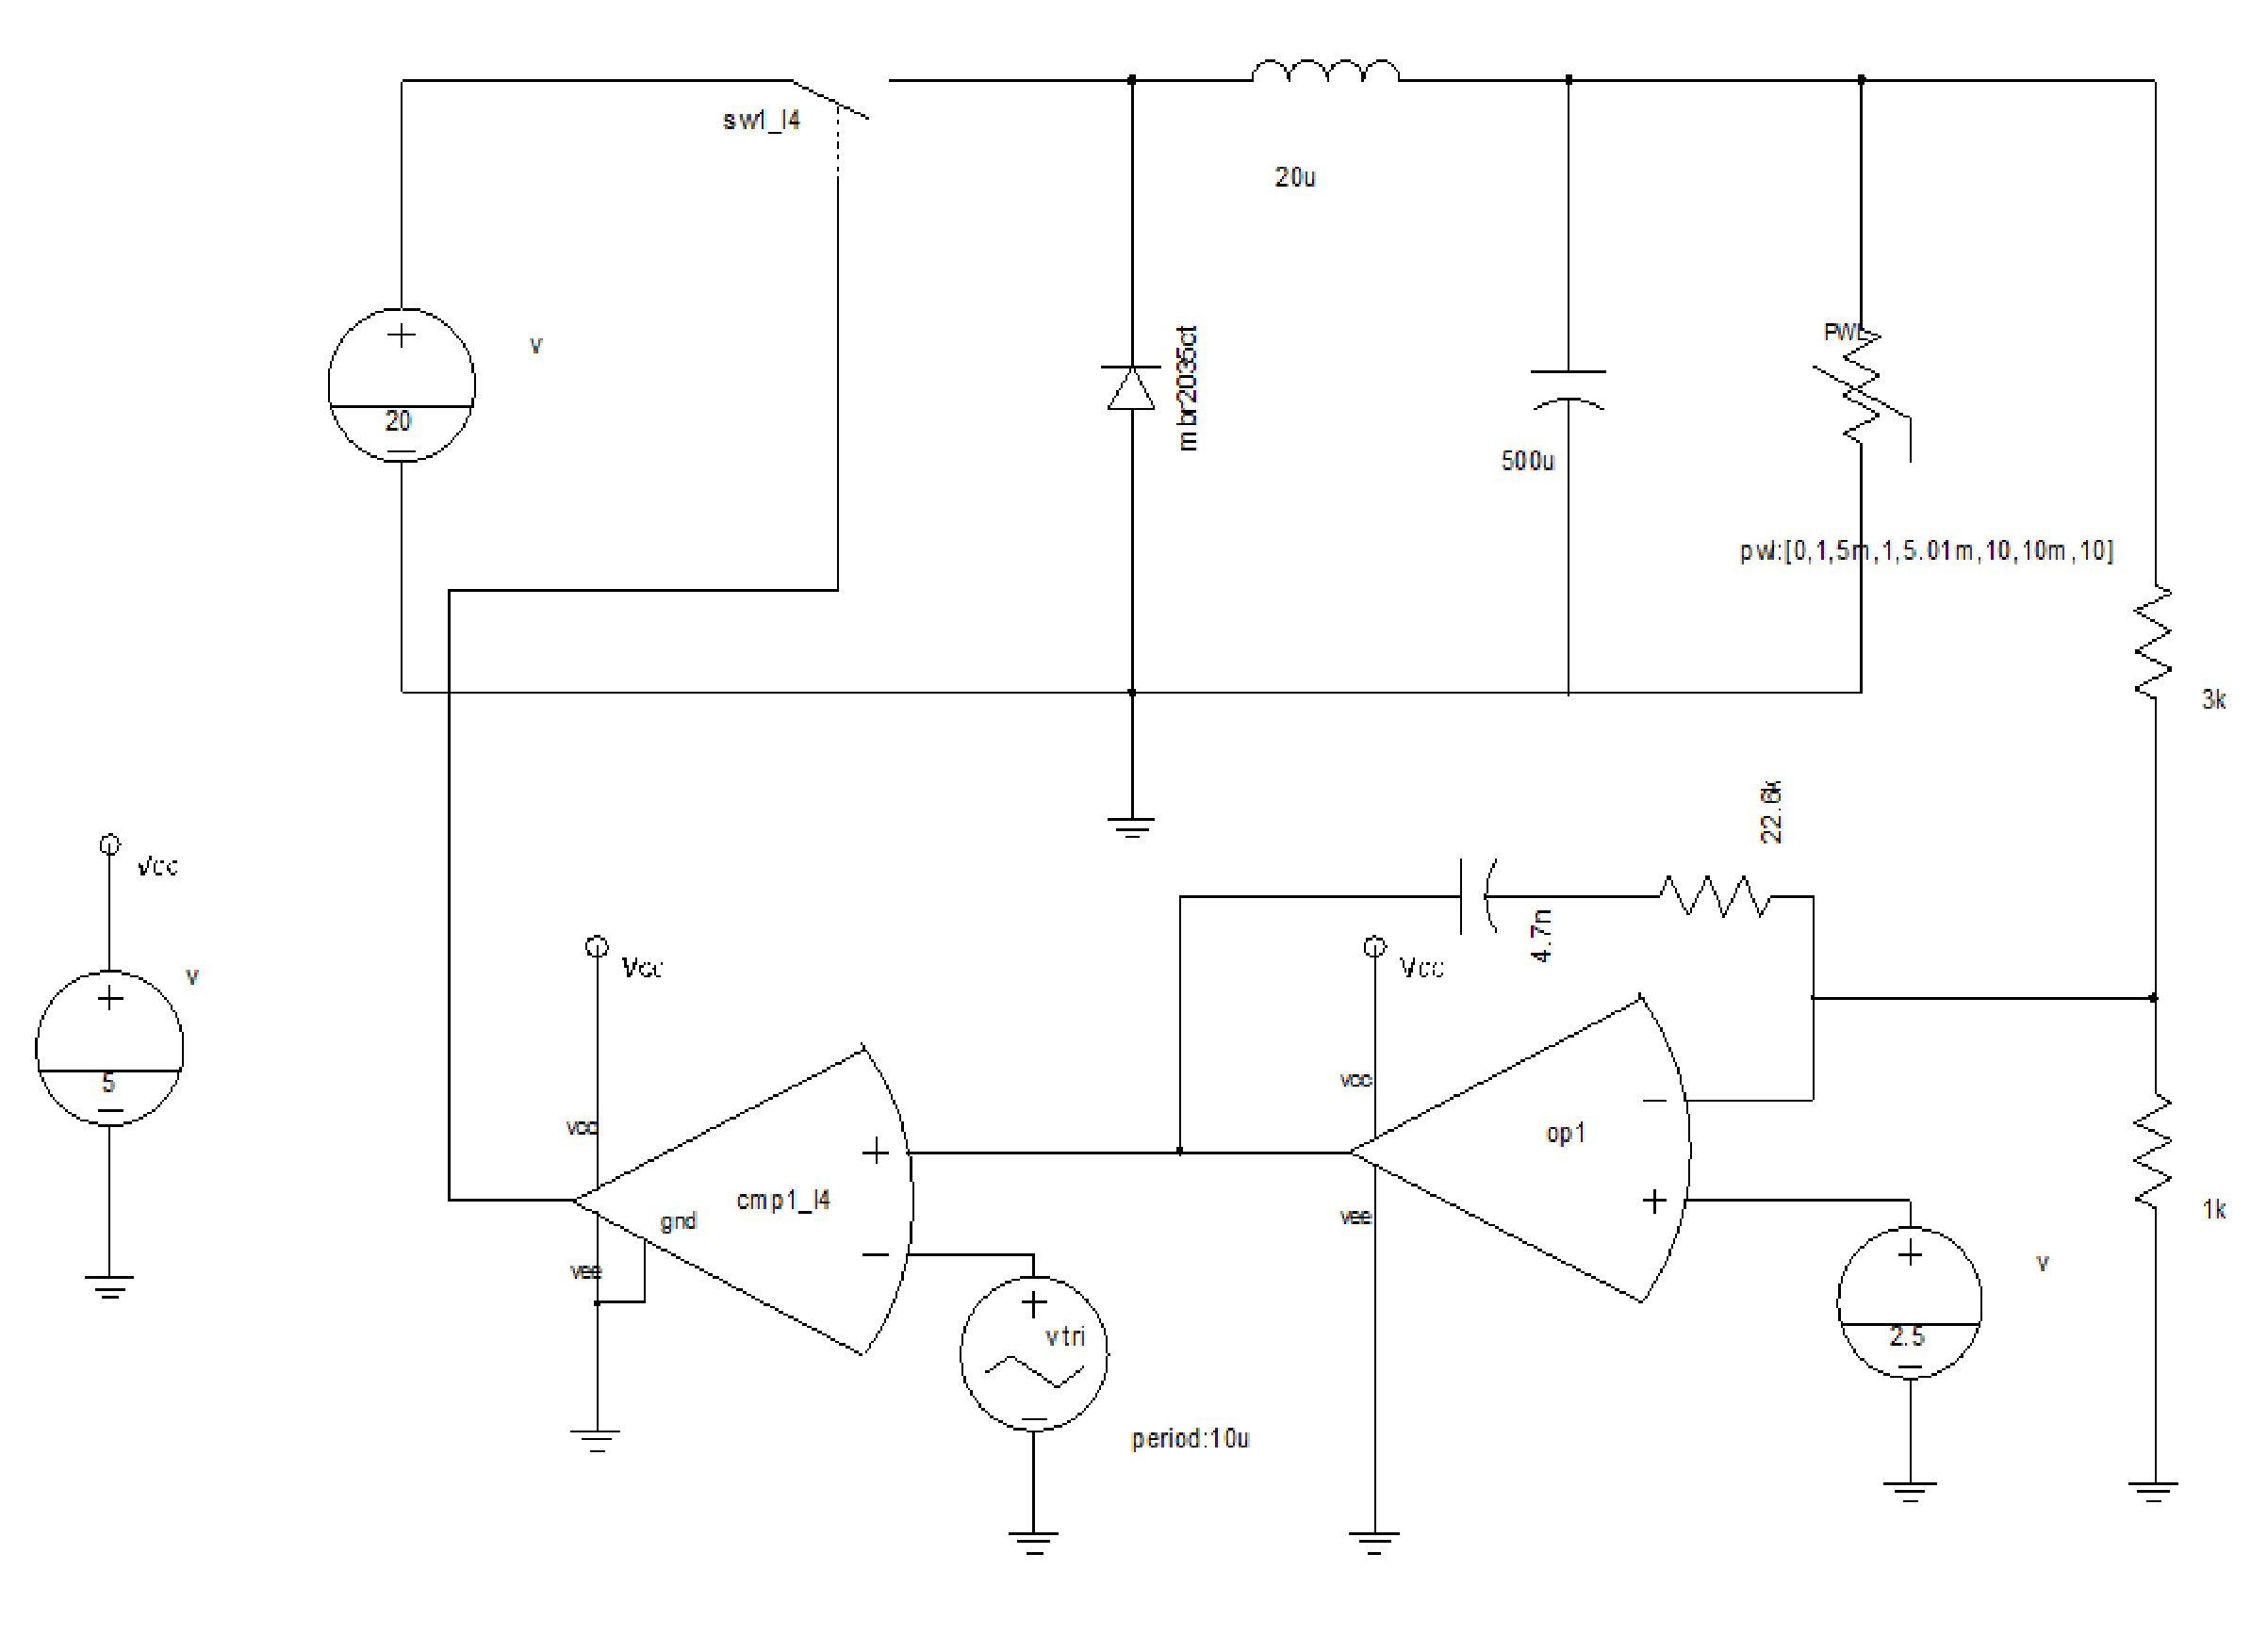
\includegraphics[width=12cm]{BuckCloseloop.pdf}\\
  %\includegraphics[width=12cm]{test_speed_step.png}\\
  \caption{基于~Buck~变换器空间电源系统~Saber~仿真图}\label{fig:chap5:buckcloseloop}
\end{figure}
\fi
\begin{figure}[h]
\begin{minipage}[t]{0.5\linewidth}
  \centering
  % Requires \usepackage{graphicx}
  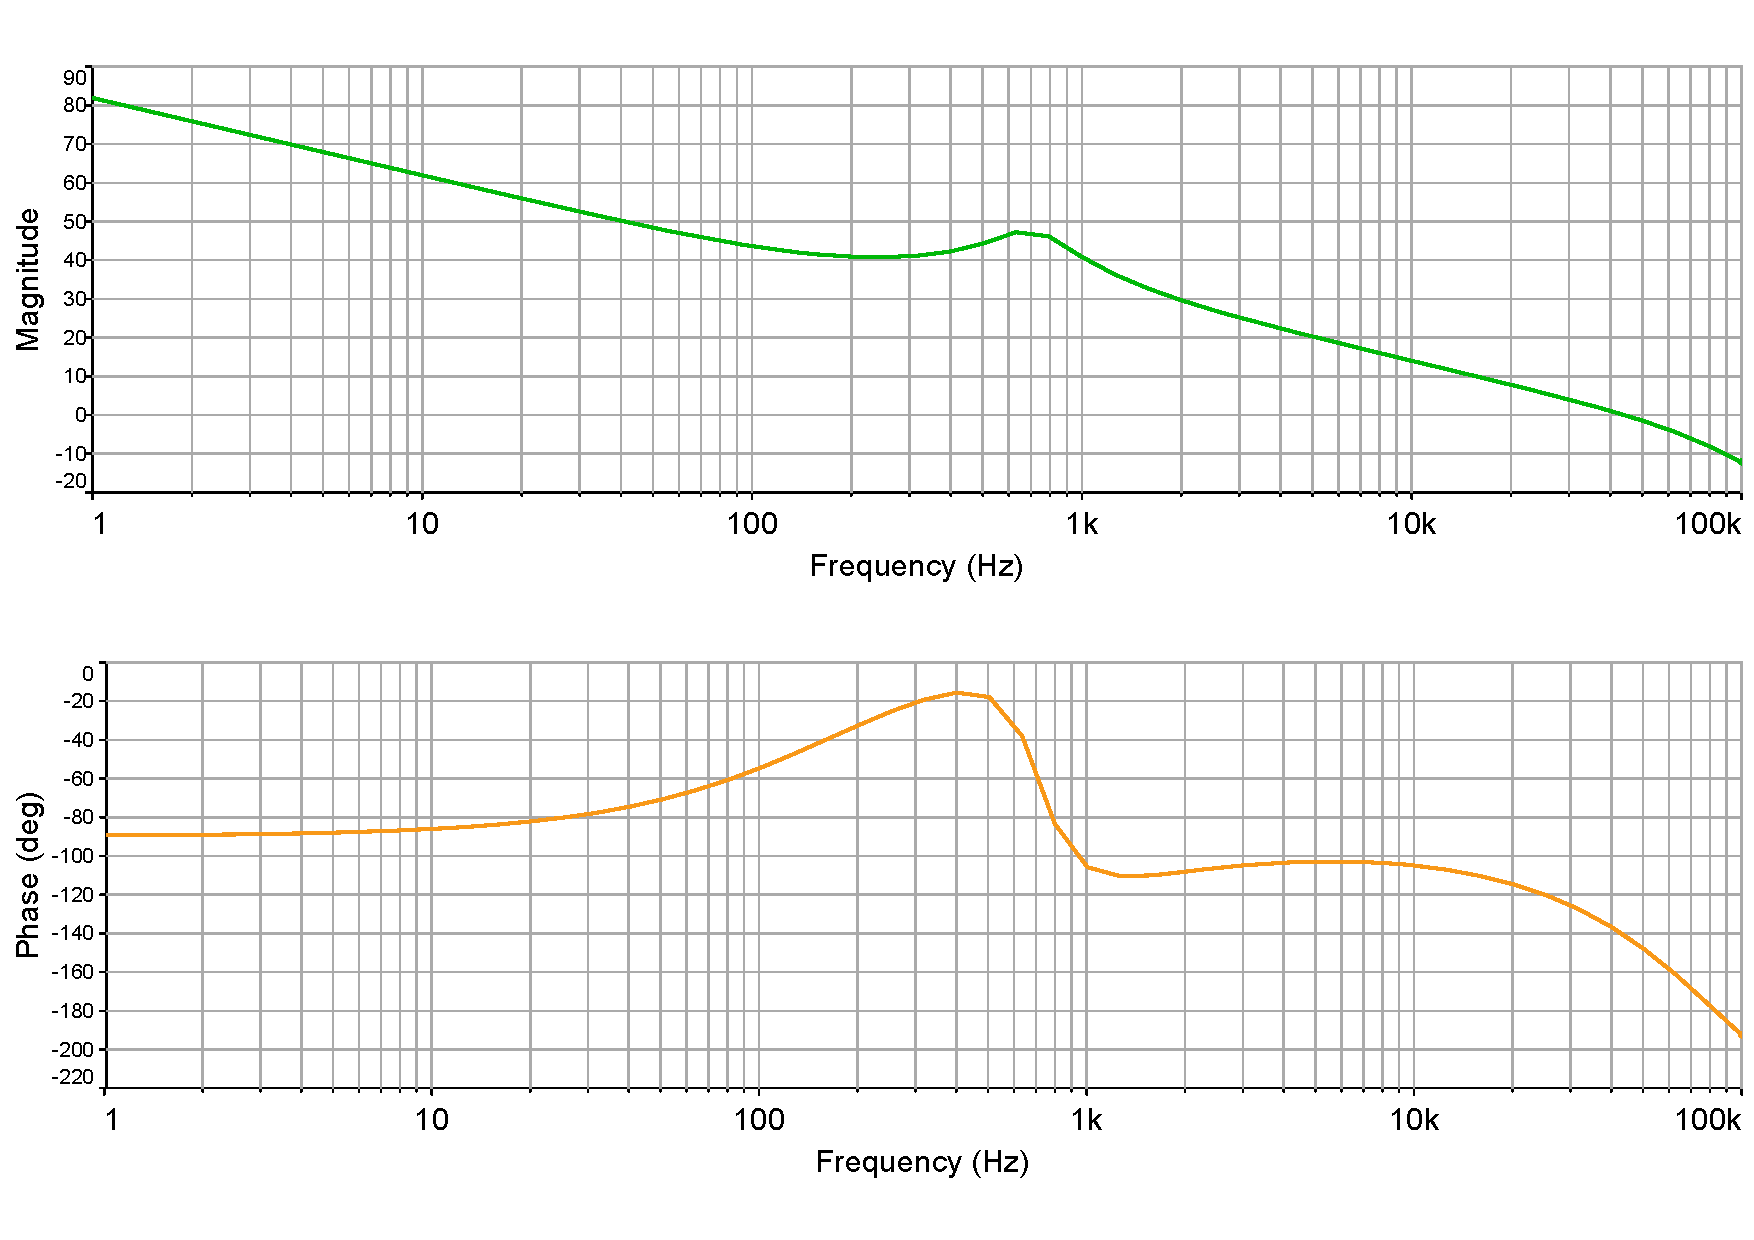
\includegraphics[height=6cm,width=7cm]{Bode.pdf}\\
  \caption{电源系统的频率特性曲线}\label{fig:chap5:bodegraph}
\end{minipage}
\begin{minipage}[t]{0.5\linewidth}
  \centering
  % Requires \usepackage{graphicx}
  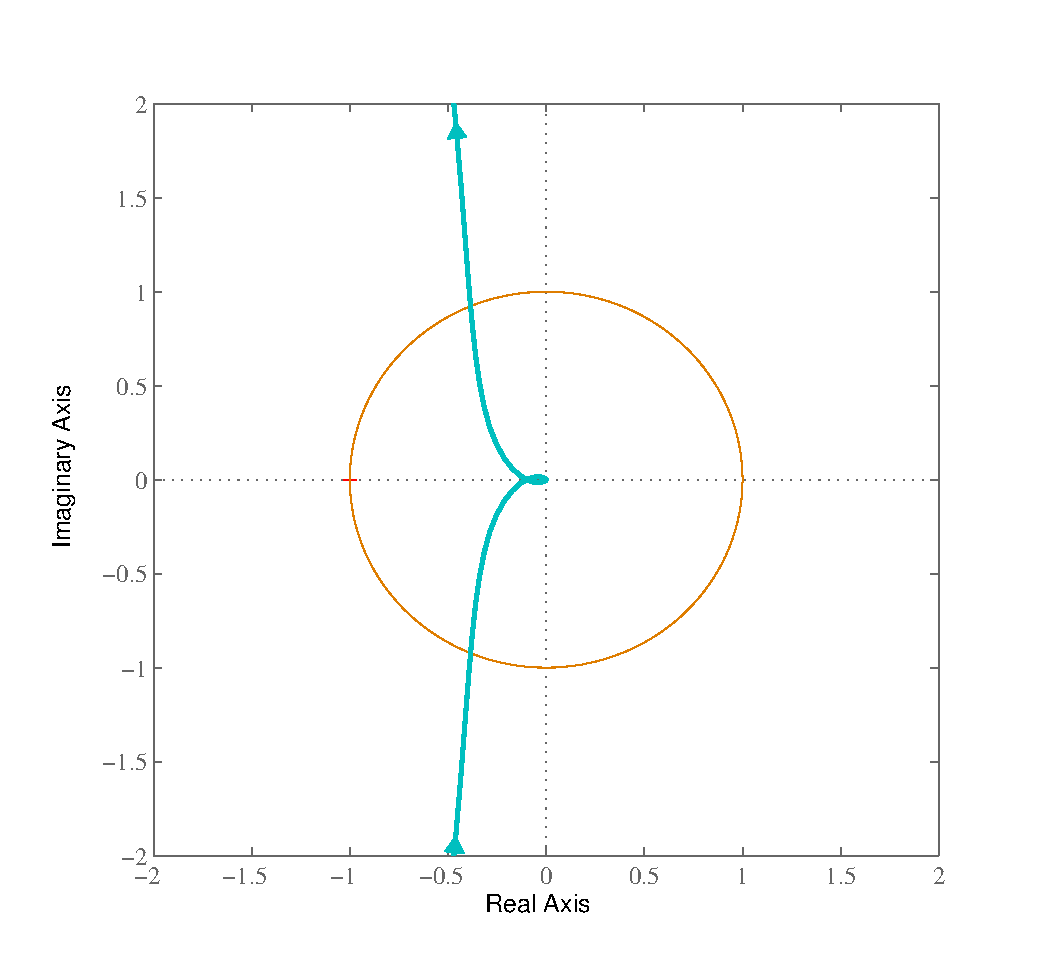
\includegraphics[height=6.5cm,width=7cm]{Nyquist.pdf}\\
  \caption{电源系统的奈奎斯特曲线}\label{fig:chap5:nyquist}
\end{minipage}
\end{figure}

\newpage
将基于~Buck~变换器的电源系统电路拓扑图转化为控制框图,通过小信号建模等效分析系统控制框图中每个环节的传递函数,推导出基于~Buck~变换器电源系统的整体传递函数。
\begin{figure}[h]
  \centering
  % Requires \usepackage{graphicx}
     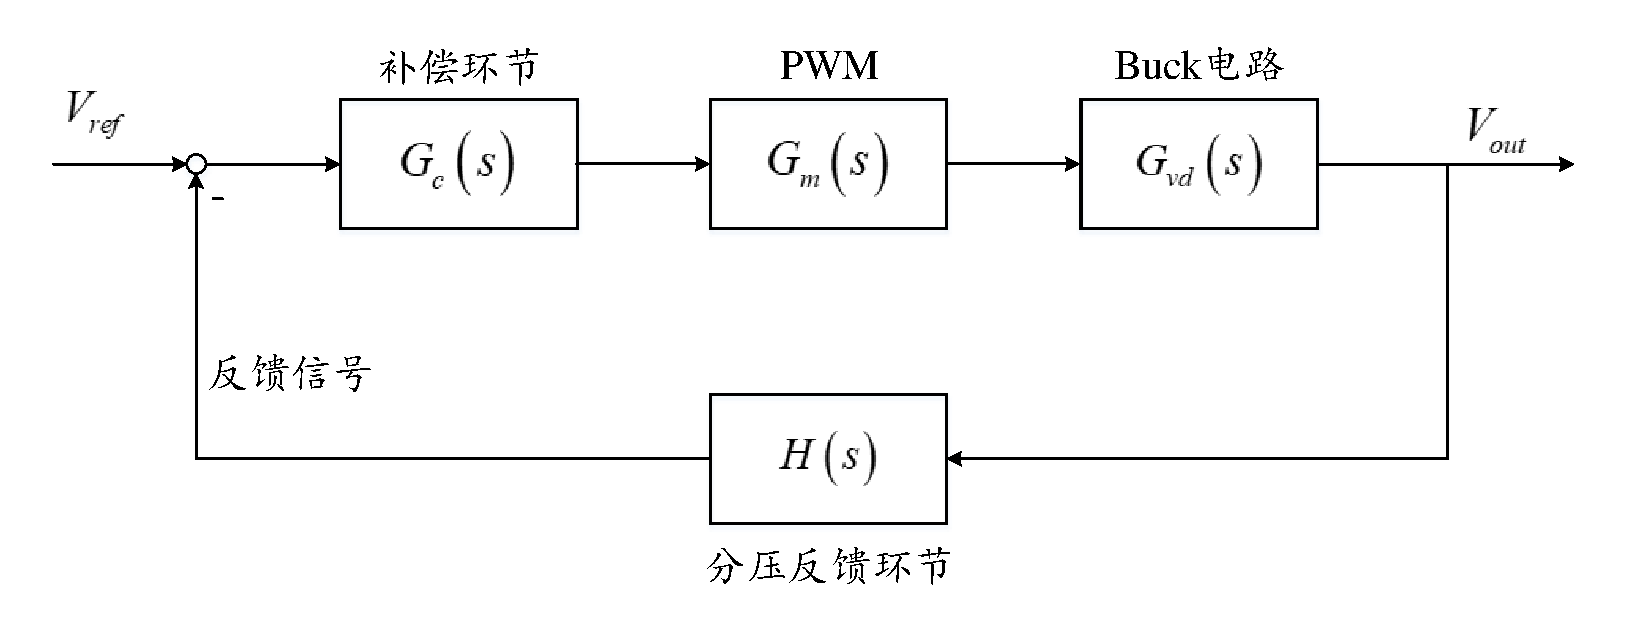
\includegraphics[width=12cm]{KongzhiKuangtu.pdf}\\
  %\includegraphics[width=12cm]{test_speed_step.png}\\
  \caption{基于~Buck~变换器电源系统的控制框图}\label{fig:chap5:kongzhikuangtu}
\end{figure}

经过推导,可得基于~Buck~变换器电源系统控制框图中:

Buck~变换器的传递函数~$G_{vd}\left(s\right)$~为
%强制改变字体大小使得分子分母字体大小一致
% \newcommand{\FS}[2]{\displaystyle\frac{#1}{#2}}
 %%%%%%%%%%%%%%%%%%%%%%%%%
\begin{equation}\label{equ:chap5:Index1}
  G_{vd}\left(s\right)=\FS{V_{out}}{D}\cdot\FS{1}{s^2LC+{s}\FS{L}{R_L}+1}
\end{equation}

式中~$R_L$~、~L~、~C~为~Buck~变换器的元件参数,~D~为输出稳定电压时~PWM~波占空比。
补偿环节的传递函数~$G_c\left(s\right)$~为
\begin{equation}\label{equ:chap5:Index2}
  G_{c}\left(s\right)=\FS{\left(1+sR_2C_1\right)\cdot\left[1+s\left(R_1+R_3\right)C_3\right]}{\left[sR_1\left(C_1+C_2\right)\right]\cdot\left[1+s\FS{R_2C_1C_2}{C_1+C+2}\right]\cdot\left(1+sR_3C_3\right)}
\end{equation}

式中~$R_1$~、~$R_2$~、~$R_3$~、~$C_1$~、~$C_2$~、~$C_3$~分别为补偿环节的元件参数。

PWM~调制环节的传递函数~$G_m\left(s\right)$~为
\begin{equation}\label{equ:chap5:Index3}
  G_{m}\left(s\right)=\FS{1}{V_m}
\end{equation}

式中~$V_m$~为~PWM~调制器锯齿波幅度。\\
\medskip

分压反馈环节的传递函数~$H\left(s\right)$~为
%\begin{small}
\begin{equation}\label{equ:chap5:Index4}
  H\left(s\right)=\FS{R_y}{R_x+R_y}
\end{equation}
%\end{small}

式中~$R_x$~与~$R_y$~分别为分压反馈环节中的电阻元件参数。
\medskip

基于~Buck~变换器电源系统的开环传递函数~$G_o\left(s\right)$~为
\begin{small}
\begin{equation}\label{equ:chap5:Index5}
\begin{split}
 &  G_o\left(s\right) ={G_c\left(s\right)}\cdot{G_m\left(s\right)}\cdot{G_{vd}\left(s\right)}\cdot{H\left(s\right)} \\
     &=\FS{\left(1+sR_2C_1\right)\cdot\left[1+s\left(R_1+R_2\right)C_3\right]\cdot{R_yV_{out}}}{\left[{sR_1}\cdot\left(C_1+C_2\right)\right]\cdot\left[1+s\FS{R_2C_1C_2}{C_1+C_2}\right]\cdot\left(1+sR_3C_3\right)\cdot{V_m}\cdot\left(R_x+R_y\right)\cdot{D}\cdot\left(s^2LC+s\FS{L}{R_L}+1\right)}
\end{split}
\end{equation}
\end{small}

系统的灵敏度函数~$S\left(s\right)$~为
\begin{small}
\begin{equation}\label{equ:chap5:Index6}
\begin{split}
 &  S_s\left(s\right) =\FS{1}{1+{G_c\left(s\right)}\cdot{G_m\left(s\right)}\cdot{G_{vd}\left(s\right)}\cdot{H\left(s\right)}}\\
     &=\FS{1}{1+\FS{\left(1+sR_2C_1\right)\cdot\left[1+s\left(R_1+R_3\right)C_3\right]}{\left[{sR_1}\cdot\left(C_1+C_2\right)\cdot\left[1+s\FS{R_2C_1C_2}{C_1+C_2}\right]\cdot\left(1+sR_3C_3\right)\cdot{V_m}\right]}\cdot\FS{V_{out}}{D}\cdot\FS{1}{s^2LC+{s}\FS{L}{R_L}+1}\cdot\FS{R_y}{R_x+R_y}}
\end{split}
\end{equation}
\end{small}
%\left[\right]
%\medskip     行间距微调

\subsection{基于~Buck~变换器空间电源系统电子元件模型}
\label{sub:chap5:step}
由第二章对恶劣工作环境中电子元器件的建模分析可知,空间电源电子元件在太空工作时主要受到温度与辐射的影响。由于~PWM~信号脉冲宽度调制环节以及电路补偿环节为小功率控制部分,为保证~PWM~波控制信号的精度,对控制部分电路中的电子元件通常会采取温度补偿以及电磁屏蔽措施。在高可靠领域,脉冲宽度调制环节经常采用高精度、高可靠的数字芯片来实现,增强对噪声的抵抗能力。因此,本文中只考虑~Buck~变换器主拓扑中电子元件随恶劣环境影响而产生的元件参数变化。

空间电源~Buck~变换器主拓扑中电阻~$R_L$~为~$1\Omega$~,滤波电感~$L$~为~$0.1mH$~,滤波电容~$C$~为~$500\mu F$~,在极端辐射环境中电阻参数随温度~T~变化的数学模型为
\begin{equation}\label{equ:chap5:Index7}
  R=1.0086\cdot\left[1+0.00393\cdot\left(T-20\right)\right]
\end{equation}

极端辐射环境中电容参数随温度~T~变化的数学模型为
\begin{equation}\label{equ:chap5:Index8}
\begin{split}
   C & =0.83\times500\times10^{-6}\times\left(1+\Delta C\right) \\
      & =4.15\times10^{-4}\cdot\left(1+\Delta C\right)
\end{split}
\end{equation}

$\Delta C$为由温度引起的电容变化值,由多项式表示
\begin{equation}\label{equ:chap5:Index9}
  \Delta C=f\left(T\right)\times 100\%=p_1\cdot T^7+p_2\cdot T^6+p_3\cdot T^5+p_4\cdot T^4+p_5\cdot T^3+p_6\cdot T^2+p_7\cdot T+p_8
\end{equation}	

多项式参数为

\qquad \qquad $p_1=-1.569\times 10^{-16}$     \qquad \qquad ~$p_5= 1.780\times 10^{-7} $

\qquad \qquad  $p_2= 1.085\times 10^{-13}$    \qquad \qquad ~~~$p_6=-1.461\times 10^{-5}$

\qquad \qquad $p_3=-2.215\times 10^{-11}$     \qquad \qquad $p_7= 0.487\times 10^{-4}$

\qquad \qquad $p_4= 5.817\times 10^{-10}$     \qquad \qquad ~~~$ p_8=-0.01$
\iffalse
\begin{table}[htbp]
  \centering
\begin{tabular}{p{5cm}p{5cm}}

  $p_1=-1.569\times 10^{-16}$     & $p_5= 1.780\times 10^{-7} $\\

  $p_2= 1.085\times 10^{-13}$     & $p_6=-1.461\times 10^{-5}$ \\

  $p_3=-2.215\times 10^{-11}$     & $p_7= 0.487\times 10^{-4}$ \\

 $p_4= 5.817\times 10^{-10}$      & $ p_8=-0.01$ \\

\end{tabular}
%  \caption{}\label{tab:chap5:canshu}
\end{table}
\fi

极端辐射环境中电感参数值随温度~T~变化的数学模型为
\begin{equation}\label{equ:chap5:Index10}
  L=0.1\times 10^{-3}\cdot\left[1+88\times 10^{-6}\cdot\left(T-20\right)\right]
\end{equation}

\section{基于~Buck~变换器空间电源系统不确定性建模}
\label{sub:chap5:compare}
实际空间电源系统由于工作环境、设备装配方式以及元件自身参数变化会使系统模型产生不确定性,这些不确定性的存在正是导致系统脆弱性的关键原因。在进行基于~Buck~变换器的空间电源系统脆弱性分析之前,需要分别建立系统中电阻、电容、电感元件有界的加性不确定性系统模型,采用数学的方式描述系统的不确定性。

本文中将补偿电路环节、分压反馈环节以及~PWM~信号脉冲宽度调制环节中的电子元件作为理想电子元件考虑,空间电源系统的不确定性主要体现在~Buck~变换器电路上,具有不确定性的系统控制框图如图~\ref{fig:chap5:adduncertainty}~所示,其中$\Delta\left(s\right)$为规范化不确定性,$W\left(s\right)$为加权函数。
\begin{figure}[h]
  \centering
  % Requires \usepackage{graphicx}
     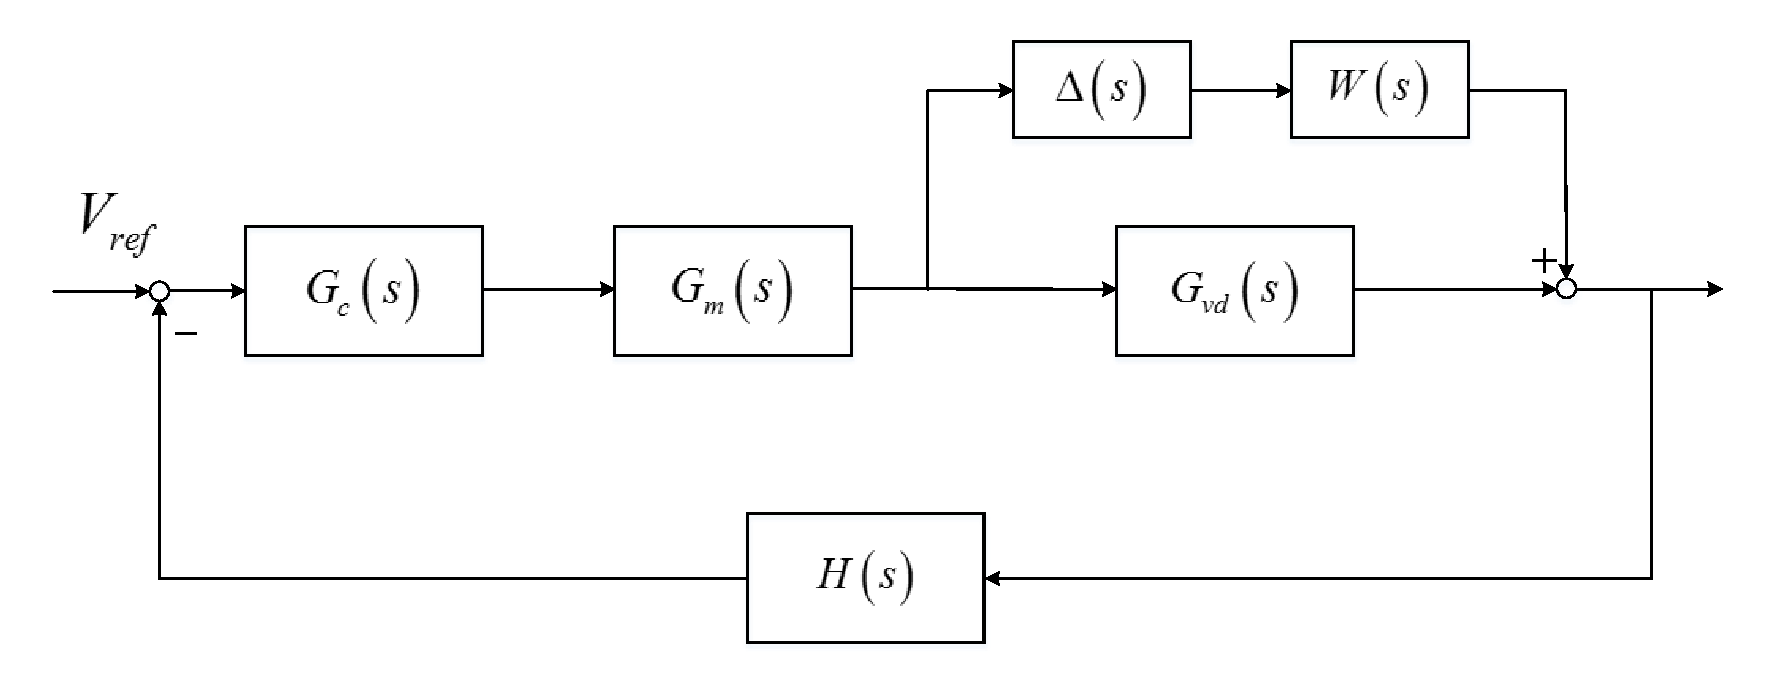
\includegraphics[width=11cm]{AddUncertainty.pdf}\\
  %\includegraphics[width=12cm]{test_speed_step.png}\\
  \caption{具有加性不确定性的空间电源系统}\label{fig:chap5:adduncertainty}
\end{figure}

\subsection{电阻元件不确定时系统建模}
\label{sub:chap5:R_uncertainty}

当空间电源~Buck~变换器主拓扑中的电阻元件参数~$R^{\prime}$~在~$R_{min}$~与~$R_{max}$~之间波动,实际~Buck~变换器~$G_R\left(s\right)$~属于非结构化集合
\begin{equation}\label{equ:chap5:Index11}
 U_{R}=\left\{G_{R}\left(s\right)=G_{vd}\left(s\right)+W_{R}\left(s\right)\cdot \Delta\left(s\right):\Delta\left(s\right) \in  \overline{BH_{\infty}}\right\}
\end{equation}

经公式推导可以得出描述电阻元件不确定性的表达式~$W_{R}\left(s\right)\cdot\Delta\left(s\right)$~为
\begin{equation}\label{equ:chap5:Index12}
W_{R}\left(s\right)\cdot\Delta\left(s\right)=\FS{V_{out}}{D}\cdot\left(\FS{sL\cdot\left(R-R^{\prime}\right)}{\left(s^2R^{\prime}LC+sL+R^{\prime}\right)\cdot\left(s^2RLC+sL+R\right)}\right)
\end{equation}

由$\left|\Delta\left(jw\right)\right|\leqslant 1$可得
\begin{equation}\label{equ:chap5:Index13}
\left|W_R\left(jw\right) \right|=\left|  \FS{V_{out}}{D}\cdot\left(\FS{jwL\cdot\left(R-R^{\prime}\right)}{\left(\left(jw\right)^2R^{\prime}LC+jwL+R^{\prime}\right)\cdot\left(\left(jw\right)^2RLC+jwL+R\right)}\right)
 \right|_{max}
\end{equation}

结合~Buck~变换器的传递函数~$G_{vd}\left(s\right)$、补偿环节的传递函数~$G_{c}\left(s\right)$、PWM~调制环节的传递函数~$G_{m}\left(s\right)$~以及分压反馈环节的传递函数~$H\left(s\right)$,可以得到电阻元件不确定时系统的数学模型。

\subsection{电容元件不确定时系统建模}
\label{sub:chap5:C_uncertainty}

当空间电源~Buck~变换器主拓扑中的电容元件参数~$C^{\prime}$~在~$C_{min}$~与~$C_{max}$~之间波动,实际~Buck~变换器~$G_C\left(s\right)$~属于非结构化集合
\begin{equation}\label{equ:chap5:Index14}
 U_{C}=\left\{G_{C}\left(s\right)=G_{vd}\left(s\right)+W_{C}\left(s\right)\cdot \Delta\left(s\right):\Delta\left(s\right) \in  \overline{BH_{\infty}}\right\}
\end{equation}

经公式推导可以得出描述电容元件不确定性的表达式~$W_{C}\left(s\right)\cdot\Delta\left(s\right)$~为
\begin{equation}\label{equ:chap5:Index15}
W_{C}\left(s\right)\cdot\Delta\left(s\right)=\FS{V_{out}}{D}\cdot\left(\FS{s^2L\cdot\left(C-C^{\prime}\right)}{\left(s^2LC^{\prime}+s\FS{L}{R}+1\right)\cdot\left(s^2LC+s\FS{L}{R}+1\right)}\right)
\end{equation}

由~$\left|\Delta\left(jw\right)\right|\leqslant 1$~可得
\begin{equation}\label{equ:chap5:Index16}
\left|W_C\left(jw\right) \right|=\left|  \FS{V_{out}}{D}\cdot\left(\FS{\left(jw\right)^2L\cdot\left(C-C^{\prime}\right)}{\left(\left(jw\right)^2LC^{\prime}+jw\FS{L}{R}+1\right)\cdot\left(\left(jw\right)^2LC+jw\FS{L}{R}+1\right)}\right)
 \right|_{max}
\end{equation}

结合~Buck~变换器的传递函数~$G_{vd}\left(s\right)$、补偿环节的传递函数~$G_{c}\left(s\right)$、PWM~调制环节的传递函数~$G_{m}\left(s\right)$~以及分压反馈环节的传递函数~$H\left(s\right)$,可以得到电容元件不确定时系统的数学模型。

\subsection{电感元件不确定时系统建模}
\label{sub:chap5:C_uncertainty}

当空间电源~Buck~变换器主拓扑中的电感元件参数~$L^{\prime}$~在~$L_{min}$~与~$L_{max}$~之间波动,实际~Buck~变换器~$G_L\left(s\right)$~属于非结构化集合
\begin{equation}\label{equ:chap5:Index17}
 U_{L}=\left\{G_{L}\left(s\right)=G_{vd}\left(s\right)+W_{L}\left(s\right)\cdot \Delta\left(s\right):\Delta\left(s\right) \in  \overline{BH_{\infty}}\right\}
\end{equation}

经公式推导可以得出描述电感元件不确定性的表达式~$W_{L}\left(s\right)\cdot\Delta\left(s\right)$~为
\begin{equation}\label{equ:chap5:Index18}
W_{L}\left(s\right)\cdot\Delta\left(s\right)=\FS{V_{out}}{D}\cdot\left(\FS{s^2C+\FS{s}{R}\cdot\left(L-L^{\prime}\right)}{\left(s^2C^{\prime}L+s\FS{L^{\prime}}{R}+1\right)\cdot\left(s^2CL+s\FS{L}{R}+1\right)}\right)
\end{equation}

由~$\left|\Delta\left(jw\right)\right|\leqslant 1$~可得
\begin{equation}\label{equ:chap5:Index19}
\left|W_L\left(jw\right) \right|=\left|  \FS{V_{out}}{D}\cdot\left(\FS{\left(jw\right)^2C+\FS{jw}{R}\cdot\left(L-L^{\prime}\right)}{\left(\left(jw\right)^2C^{\prime}L+jw\FS{L^{\prime}}{R}+1\right)\cdot\left(\left(jw\right)^2CL+jw\FS{L}{R}+1\right)}\right)
 \right|_{max}
\end{equation}

结合~Buck~变换器的传递函数~$G_{vd}\left(s\right)$、补偿环节的传递函数~$G_{c}\left(s\right)$、PWM~调制环节的传递函数~$G_{m}\left(s\right)$~以及分压反馈环节的传递函数~$H\left(s\right)$,可以得到电感元件不确定时系统的数学模型。

\section{基于~Buck~变换器空间电源系统鲁棒稳定裕度分析}
根据第三章中控制系统脆弱性理论分析,控制系统脆弱性体现在不同工作环境中系统鲁棒稳定裕度参数~$\gamma$~的变化趋势。在分析与量化评估基于~Buck~变换器的空间电源系统脆弱性之前,需要分析空间电源系统在不同工作环境中系统的鲁棒稳定裕度 。分别对~Buck~变换器主拓扑电路中电阻、电容以及电感元件存在不确定性的情况进行分析,计算系统鲁棒稳定裕度参数~$\gamma$~的数学表达式并结合第二章所建立的空间电源电子元器件数学模型,分析在工作环境变化时系统鲁棒稳定裕度~$\gamma$~的变化趋势。

空间电源电路由于其高可靠性的应用背景,选用的电子元器件均为军用级别,具有较高的可靠性。在军用标准~GJB/Z299C-2006~电子设备可靠性预计手册中,军用级别电子元件的误差均为~$\pm5\%$~\cite{GJB}。但由于设备在安装与调试过程中会遇到特殊的工作情况,如设备长时间工作在大型感性负载旁边或电源设备安装在大型金属板旁等,会使得空间电源电路存在更大的不确定性。考虑到空间电源电路的高可靠性,本文在分析空间电源系统脆弱性时将电子元件参数值的误差取~$\pm10\%$~,具体元件参数如表~\ref{tab:chap5:circuitcanshu}~所示。
\begin{table}[htbp]
   \centering
   \caption{电子元器件的参数值}
   \label{tab:chap5:circuitcanshu}
      \begin{tabular}{C{3cm}p{3cm}p{3cm}}
      \toprule
         元器件          & 标称参数       &实际参数\\
      \midrule
        $R$               & $1\Omega$     & $\left[0.9,~~1.1\right]\Omega$\\

       $L$               & $0.1mH$         &$\left[0.09,~~0.11\right]mH$\\

       $C$                & $500\mu F$   &$\left[450,~~550\right]\mu F$\\
     \bottomrule
\end{tabular}
\end{table}

\subsection{电容元件不确定时系统鲁棒稳定裕度分析}
\label{sub:chap5:C_robust}
基于~5.3~节建立的电容不确定时的系统模型,根据第三章中对控制系统鲁棒稳定裕度的定义与分析,通过公式推导并借助~MATLAB~软件计算,分析系统在不同工作环境中的鲁棒稳定裕度参数~$\gamma$~。故基于~Buck~变换器的空间电源系统在电容元件不确定时,系统鲁棒稳定裕度分析的具体过程包含以下步骤~:

(1)~计算电容元件不确定性的加权函数~$W_C\left(s\right)$~的模值。由于~Buck~变换器主拓扑中的电容参数~$ C^{\prime}$~在~$450\mu F$~与~$550\mu F$~之间波动,根据空间电源系统电容不确定性的模型,可得电容元件不确定性的加权函数~$W_C\left(s\right)$~的模值为
\begin{equation}\label{equ:chap5:Index20}
\left|W_C\left(jw\right) \right|=\left|  \FS{V_{out}}{D}\cdot\left(\FS{\left(jw\right)^2L\cdot\left(C-C^{\prime}\right)}{\left(\left(jw\right)^2LC^{\prime}+jw\FS{L}{R}+1\right)\cdot\left(\left(jw\right)^2LC+jw\FS{L}{R}+1\right)}\right)
 \right|_{max }
\end{equation}

(2)~根据鲁棒稳定裕度的计算公式可得鲁棒稳定裕度参数~$\gamma$~的表达式为
\begin{small}
\begin{equation}\label{equ:chap5:Index21}
\gamma_C=1-\left|\FS{W_C\left(jw\right)}{G_{vd}\left(jw\right)}\cdot T\left(jw\right)\right|_{max}=1-\left|\FS{G_c\left(jw\right)\cdot G_m\left(jw\right)\cdot W_C\left(jw\right)\cdot H\left(jw\right)}{1+G_c\left(jw\right)\cdot G_m\left(jw\right)\cdot W_C\left(jw\right)\cdot H\left(jw\right)}\right|_{max}
\end{equation}
\end{small}

(3)~计算系统在不同工作频率中,复频域表达式~\ref{equ:chap5:Index21}~幅值的最大值。定义该复频域表达式为系统补鲁棒稳定裕度参数~$\xi_C$,即
\begin{equation}\label{equ:chap5:Index22}
\xi_C=\FS{G_c\left(s\right)\cdot G_m\left(s\right)\cdot W_C\left(s\right)\cdot H\left(s\right)}{1+G_c\left(s\right)\cdot G_m\left(s\right)\cdot G_vd\left(s\right)\cdot H\left(s\right)}
\end{equation}

采用扫频的方式,计算系统在不同工作频率下补鲁棒稳定裕度参数~$\xi_C$~幅值的最大值,从而计算鲁棒稳定裕度参数~$\gamma_C$。图~\ref{fig:chap5:bulingmin}~所示为工作在~$20^{\circ}C$~环境中,电容元件不确定时系统补鲁棒稳定裕度参数~$\xi_C$~幅值的扫频结果。由图可知,系统补鲁棒稳定裕度参数~$\xi_C$~幅值的最大值为~0.2471,则此时系统鲁棒稳定裕度为~0.7529。
\begin{figure}[h]
  \centering
      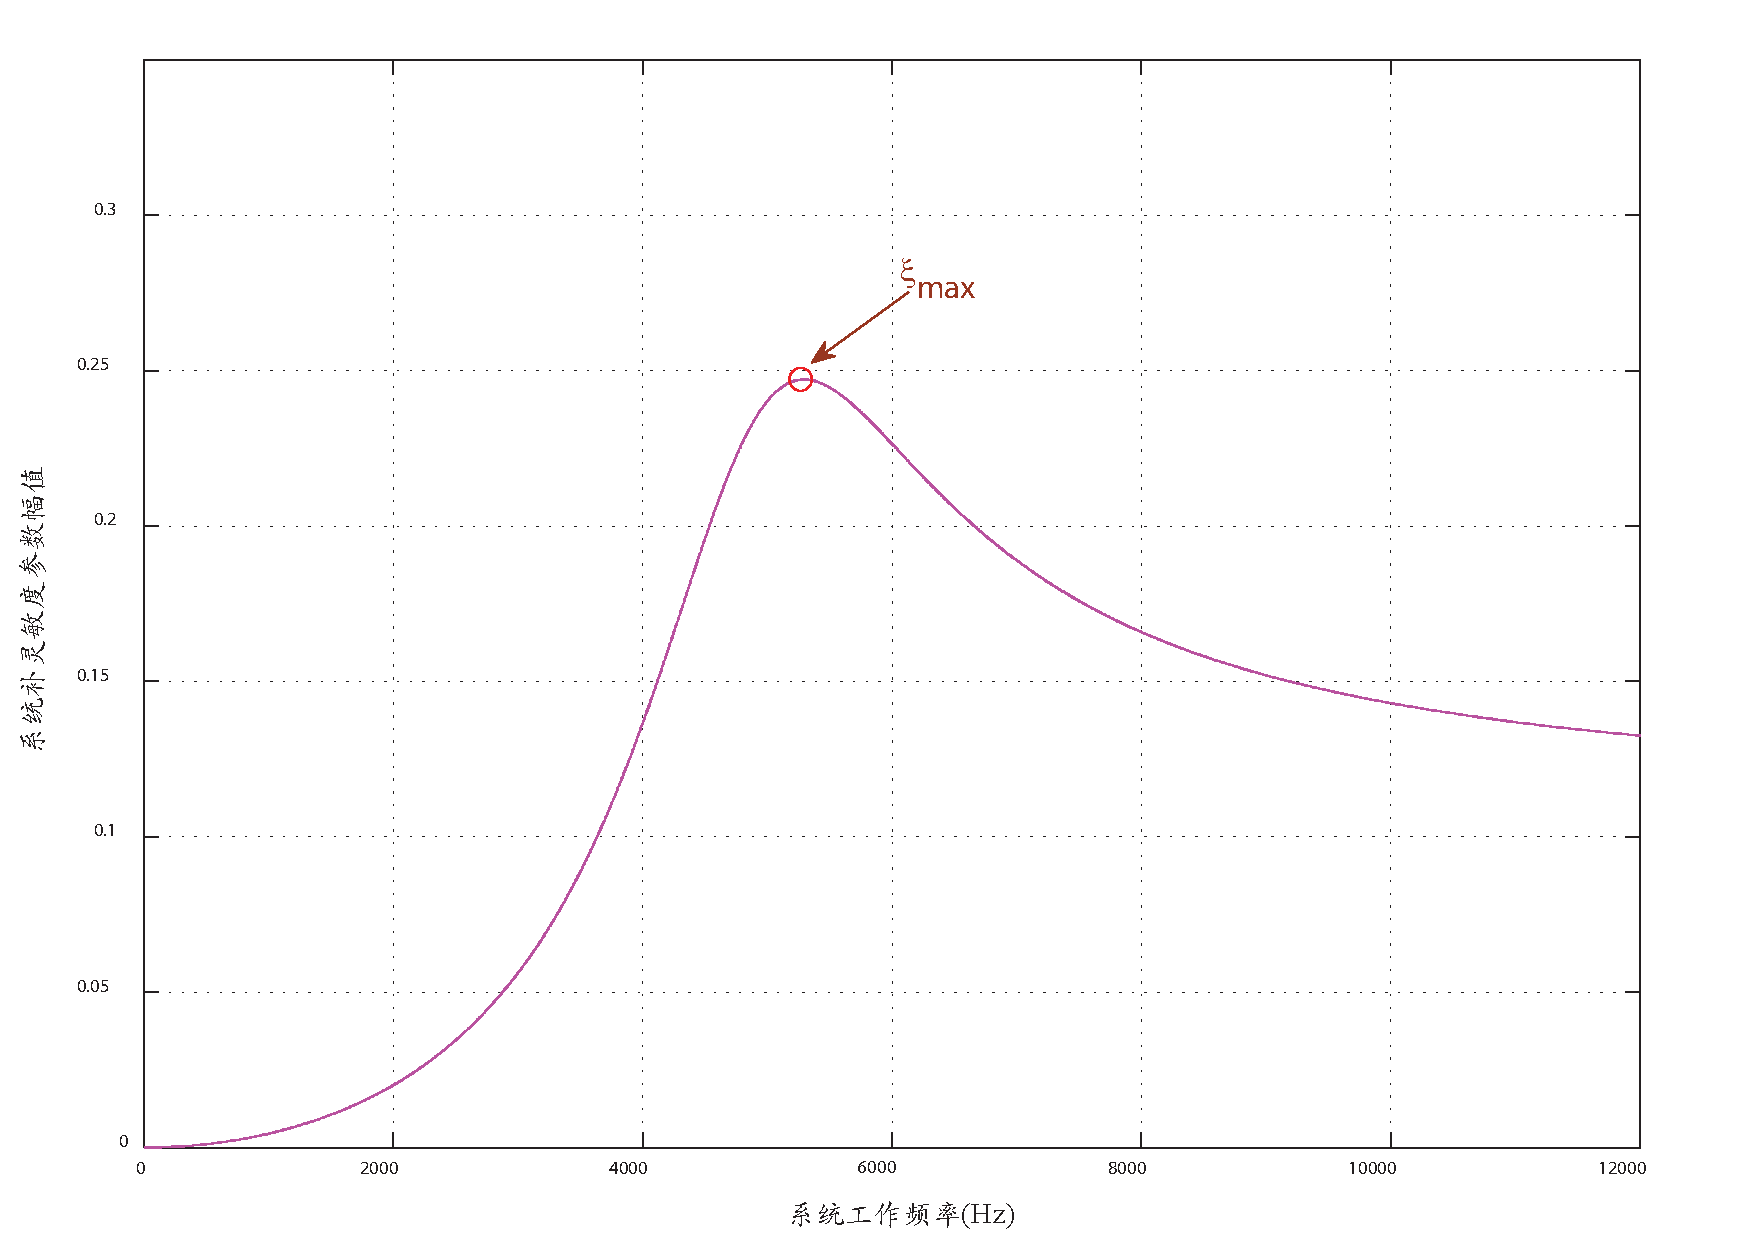
\includegraphics[width=14cm]{BuLuBang.pdf}\\
  \caption{电容元件不确定时系统补鲁棒稳定裕度~$\xi_C$}\label{fig:chap5:bulingmin}
\end{figure}

(4)~根据第二章中建立的电子元件数学模型来模拟空间电源的极端工作环境,在不同工作环境中重复第三步的扫频计算,得到在不同工作环境中系统的鲁棒稳定裕度参数~$\gamma_C$。
\subsection{电感元件不确定时系统鲁棒稳定裕度分析}
依据~5.3~节建立的电感不确定时的系统模型,基于~Buck~变换器的空间电源系统在电感元件不确定时,系统鲁棒稳定裕度分析的具体过程包含以下步骤~:

(1)~计算电感元件不确定性的加权函数~$W_L\left(s\right)$~的模值。由于~Buck~变换器主拓扑中的电感参数
~$L^{\prime}$~在~$0.09mH$~与~$0.11mH$~之间波动,根据空间电源系统电感不确定性的模型,可得电感元件不确定性的加权函数~$W_L\left(s\right)$~ 的模值为

\begin{small}
\begin{equation}\label{equ:chap5:Index23}
\left|W_L\left(jw\right) \right|=\left|  \FS{V_{out}}{D}\cdot\left(\FS{\left(jw\right)^2C+\FS{jw}{R}\cdot\left(L-L^{\prime}\right)}{\left(\left(jw\right)^2C^{\prime}L+jw\FS{L^{\prime}}{R}+1\right)\cdot\left(\left(jw\right)^2CL+jw\FS{L}{R}+1\right)}\right)
 \right|_{max }
\end{equation}
 \end{small}

(2)~根据鲁棒稳定裕度的计算公式可得鲁棒稳定裕度参数~$\gamma_L$~的表达式为
\begin{small}
\begin{equation}\label{equ:chap5:Index24}
\gamma_L=1-\left|\FS{W_L\left(jw\right)}{G_{vd}\left(jw\right)}\cdot T\left(jw\right)\right|_{max}=1-\left|\FS{G_c\left(jw\right)\cdot G_m\left(jw\right)\cdot W_L\left(jw\right)\cdot H\left(jw\right)}{1+G_c\left(jw\right)\cdot G_m\left(jw\right)\cdot W_L\left(jw\right)\cdot H\left(jw\right)}\right|_{max}
\end{equation}
\end{small}

(3)~计算在不同工作频率中,系统的补鲁棒稳定裕度参数~$\xi_L$
\begin{equation}\label{equ:chap5:Index25}
\xi_L=\FS{G_c\left(s\right)\cdot G_m\left(s\right)\cdot W_L\left(s\right)\cdot H\left(s\right)}{1+G_c\left(s\right)\cdot G_m\left(s\right)\cdot G_vd\left(s\right)\cdot H\left(s\right)}
\end{equation}

采用扫频的方式,计算系统在不同工作频率下补鲁棒稳定裕度参数~$\xi_L$~幅值的最大值,从而计算鲁棒稳定裕度参数~$\gamma_L$。

(4)~根据第二章中建立的电子元件数学模型来模拟空间电源的极端工作环境,在不同工作环境中重复第三步的扫频计算,得到在不同工作环境中系统的鲁棒稳定裕度参数~$\gamma_L$。
\subsection{电阻元件不确定时系统鲁棒稳定裕度分析}
依据~5.3~节建立的电阻不确定时的系统模型,基于~Buck~变换器的空间电源系统在电阻元件不确定时,系统鲁棒稳定裕度分析的具体过程包含以下步骤~:

(1)~计算电阻元件不确定性的加权函数~$W_R\left(s\right)$~的模值。由于~Buck~变换器主拓扑中的电阻参数~$R^ {\prime}$~在~$0.9\Omega$~与~$1.1\Omega$~之间波动,根据空间电源系统电阻不确定性的模型,可得电阻元件不确定性的加权函数~$W_R\left(s\right)$~的模值为

\begin{small}
\begin{equation}\label{equ:chap5:Index26}
\left|W_R\left(jw\right) \right|=\left|  \FS{V_{out}}{D}\cdot\left(\FS{jwL\cdot\left(R-R^{\prime}\right)}{\left(\left(jw\right)^2R^{\prime}LC+jwL+R^{\prime}\right)\cdot\left(\left(jw\right)^2RLC+jwL+R\right)}\right)
 \right|_{max}
\end{equation}
 \end{small}

(2)~根据鲁棒稳定裕度的计算公式可得鲁棒稳定裕度参数~$\gamma_R$~的表达式为
\begin{small}
\begin{equation}\label{equ:chap5:Index27}
\gamma_R=1-\left|\FS{W_R\left(jw\right)}{G_{vd}\left(jw\right)}\cdot T\left(jw\right)\right|_{max}=1-\left|\FS{G_c\left(jw\right)\cdot G_m\left(jw\right)\cdot W_R\left(jw\right)\cdot H\left(jw\right)}{1+G_c\left(jw\right)\cdot G_m\left(jw\right)\cdot W_L\left(jw\right)\cdot H\left(jw\right)}\right|_{max}
\end{equation}
\end{small}

(3)~计算在不同工作频率中,系统的补鲁棒稳定裕度参数~$\xi_R$
\begin{equation}\label{equ:chap5:Index28}
\xi_R=\FS{G_c\left(s\right)\cdot G_m\left(s\right)\cdot W_R\left(s\right)\cdot H\left(s\right)}{1+G_c\left(s\right)\cdot G_m\left(s\right)\cdot G_vd\left(s\right)\cdot H\left(s\right)}
\end{equation}

采用扫频的方式,计算系统在不同工作频率下补鲁棒稳定裕度参数~$\xi_R$~幅值的最大值,从而计算鲁棒稳定裕度参数~$\gamma_R$。

(4)~根据第二章中建立的电子元件数学模型来模拟空间电源的极端工作环境,在不同工作环境中重复第三步的扫频计算,得到在不同工作环境中系统的鲁棒稳定裕度参数~$\gamma_R$。

根据以上所述的鲁棒稳定裕度分析步骤,最终可得不同工作环境中基于~Buck~变换器的空间电源系统分别在电容、电感以及电阻元件存在不确定性时的鲁棒稳定裕度参数,具体参数如表~\ref{tab:chap5:data}~所示。
\newpage
%%%%%%%%%%%%%%%%%%可以分页显示的表格
%\iffalse
\begin{center} \tablecaption{电容、电感以及电阻元件不确定时系统鲁棒稳定裕度参数 \label{tab:chap5:data}}
\tablefirsthead{
\bottomrule
%\rowcolor[gray]{0.8}
\multicolumn{1}{c}{T$\left(^{\circ}C\right)$} &
\multicolumn{1}{c}{ $\gamma_C$}  &
\multicolumn{1}{c}{ $\gamma_L$}  &
\multicolumn{1}{c}{ $\gamma_R$} \\}
\tablehead{\multicolumn{2}{c}{
\small 续表 \ref{tab:chap5:data}} \\
\bottomrule
%\rowcolor[gray]{0.8}
\multicolumn{1}{c}{T$\left(^{\circ}C\right)$} &
\multicolumn{1}{c}{ $\gamma_C$}  &
\multicolumn{1}{c}{ $\gamma_L$}  &
\multicolumn{1}{c}{ $\gamma_R$} \\
\bottomrule}

\tabletail{\bottomrule
\multicolumn{2}{c}{\small 接下页} \\}
\tablelasttail{\bottomrule}
\begin{supertabular}{C{3cm}C{3cm}C{3cm}C{3cm}}
 \midrule
        $-60$                      & $0.8295$              & $0.7854$             & $0.9011$       \\ 

        $-50$                      & $0.8189$              & $0.7754$             & $0.9011$       \\ 

        $-40$                      & $0.8096$              & $0.7651$             & $0.9010$       \\ 

        $-30$                      & $0.7995$              & $0.7547$             & $0.9009$       \\ 

        $-20$                      & $0.7896$              & $0.7444$             & $0.9009$       \\ 

        $-10$                      & $0.7800$              & $0.7345$             & $0.9008$       \\ 

        $0$                         & $0.7707$              & $0.7248$             & $0.9008$       \\  

        $10$                      & $0.7617$              & $0.7155$             & $0.9008$        \\  

        $20$                      & $0.7529$              & $0.7063$             & $0.9007$        \\  

        $30$                      & $0.7442$              & $0.6972$             & $0.9007$        \\ 

        $40$                      & $0.7356$              & $0.6881$             & $0.9007$        \\ 

        $50$                      & $0.7269$              & $0.6789$             & $0.9007$        \\  

        $60$                      & $0.7182$              & $0.6697$             & $0.9007$        \\ 

        $70$                      & $0.7095$              & $0.6605$             & $0.9006$        \\ 

        $80$                      & $0.7009$              & $0.6514$             & $0.9006$        \\  

        $90$                      & $0.6925$              & $0.6425$             & $0.9006$        \\  

        $100$                    & $0.6846$              & $0.6340$             & $0.9006$        \\  

        $110$                    & $0.6774$              & $0.6263$             & $0.9006$        \\  

        $120$                    & $0.6711$              & $0.6196$             & $0.9006$        \\ 

        $130$                    & $0.6659$              & $0.6140$             & $0.9006$        \\  

        $140$                    & $0.6621$              & $0.6100$             & $0.9005$        \\  

        $150$                    & $0.6599$              & $0.6076$             & $0.9005$        \\ 

        $160$                    & $0.6594$              & $0.6070$             & $0.9005$        \\  

        $170$                    & $0.6606$              & $0.6083$             & $0.9005$        \\ 

        $180$                    & $0.6634$              & $0.6113$             & $0.9006$        \\ 

        $190$                    & $0.6676$              & $0.6158$             & $0.9006$        \\  

        $200$                    & $0.6729$              & $0.6215$             & $0.9006$        \\  

        $210$                    & $0.6789$              & $0.6279$             & $0.9006$        \\ 

        $220$                    & $0.6848$              & $0.6342$             & $0.9006$        \\ 

        $230$                    & $0.6902$              & $0.6400$             & $0.9006$        \\

        $240$                    & $0.6945$              & $0.6446$             & $0.9006$        \\ 

        $250$                    & $0.6978$              & $0.6480$             & $0.9006$        \\ 

        $260$                    & $0.7006$              & $0.6511$             & $0.9006$        \\  

        $270$                    & $0.7050$              & $0.6557$             & $0.9006$        \\

        $280$                    & $0.7148$              & $0.6661$             & $0.9006$        \\ 
 %   \bottomrule
\end{supertabular}
\end{center}
%\fi
%\newpage
\section{基于~Buck~变换器空间电源系统脆弱性分析与量化评估}
\label{sub:chap5:fraeva}
根据第四章中建立的脆弱性评估体系,分别量化评估基于~Buck~变换器的空间电源系统在电容不确定、电感不确定以及电阻不确定情况中鲁棒稳定裕度参数~$\gamma$~随系统工作环境改变的变化趋势,分析系统的脆弱性。
\subsection{电容元件不确定时系统脆弱性分析与量化评估}
基于上一小节通过~MATLAB~软件计算得到的空间电源系统在电容元件不确定情况下不同工作环境中系统鲁棒稳定裕度参数~$\gamma_C$~值,借助~Python~软件进行数据分析与处理,得到系统脆弱性量化评估结果。基于~Buck~变换器的空间电源系统在电容元件不确定时,系统脆弱性量化评估的具体过程包含以下步骤~:

(1)~对于电容元件不确定的情况,对~MATLAB~软件计算得到的系统鲁棒稳定裕度参数~$\gamma_C$~进行多项式拟合,拟合曲线如图~\ref{fig:chap5:cuncertainty}~所示。得到电容不确定情况下,系统鲁棒稳定裕度参数~$\gamma_C$~随温度~T$\left(^{\circ}C\right)$~变化的函数表达式
\begin{equation}\label{equ:chap5:Index29}
\begin{split}
   \gamma_C= &3.608\times10^{-17}\cdot T^7-2.65\times10^{-14}\cdot T^6+6.084\times10^{-12}\cdot T^5-3.232\times10^{-10}\cdot T^4\\
     & -2.672\times10^{-8}\cdot T^3+2.543\times10^{-6}\cdot T^2-9.02\times10^{-4}\cdot T+0.7701
\end{split}
\end{equation}

多项式拟合的参数指标为:

\qquad 误差平方和~$SSE\colon~~1.34\times10^{-5}$  \qquad 均方差~$MSE\colon~~3.84\times10^{-7} $

\qquad 均方根~$RMSE\colon~~6.196\times10^{-4}$    ~~~\qquad 确定系数~$R-square\colon~~0.9998$

\iffalse
\begin{table}[htbp]
  \centering
\begin{tabular}{p{5cm}p{5cm}}

  误差平方和~$SSE\colon~~1.34\times10^{-5}$     & ~~均方差~$MSE\colon~~3.84\times10^{-7} $\\

  均方根~$RMSE\colon~~6.196\times10^{-4}$     & ~~确定系数~$R-square\colon~~0.9998$ \\
\end{tabular}
%  \caption{}\label{tab:chap5:canshu}
\end{table}
\fi

\begin{figure}[h]
  \centering
  % Requires \usepackage{graphicx}
     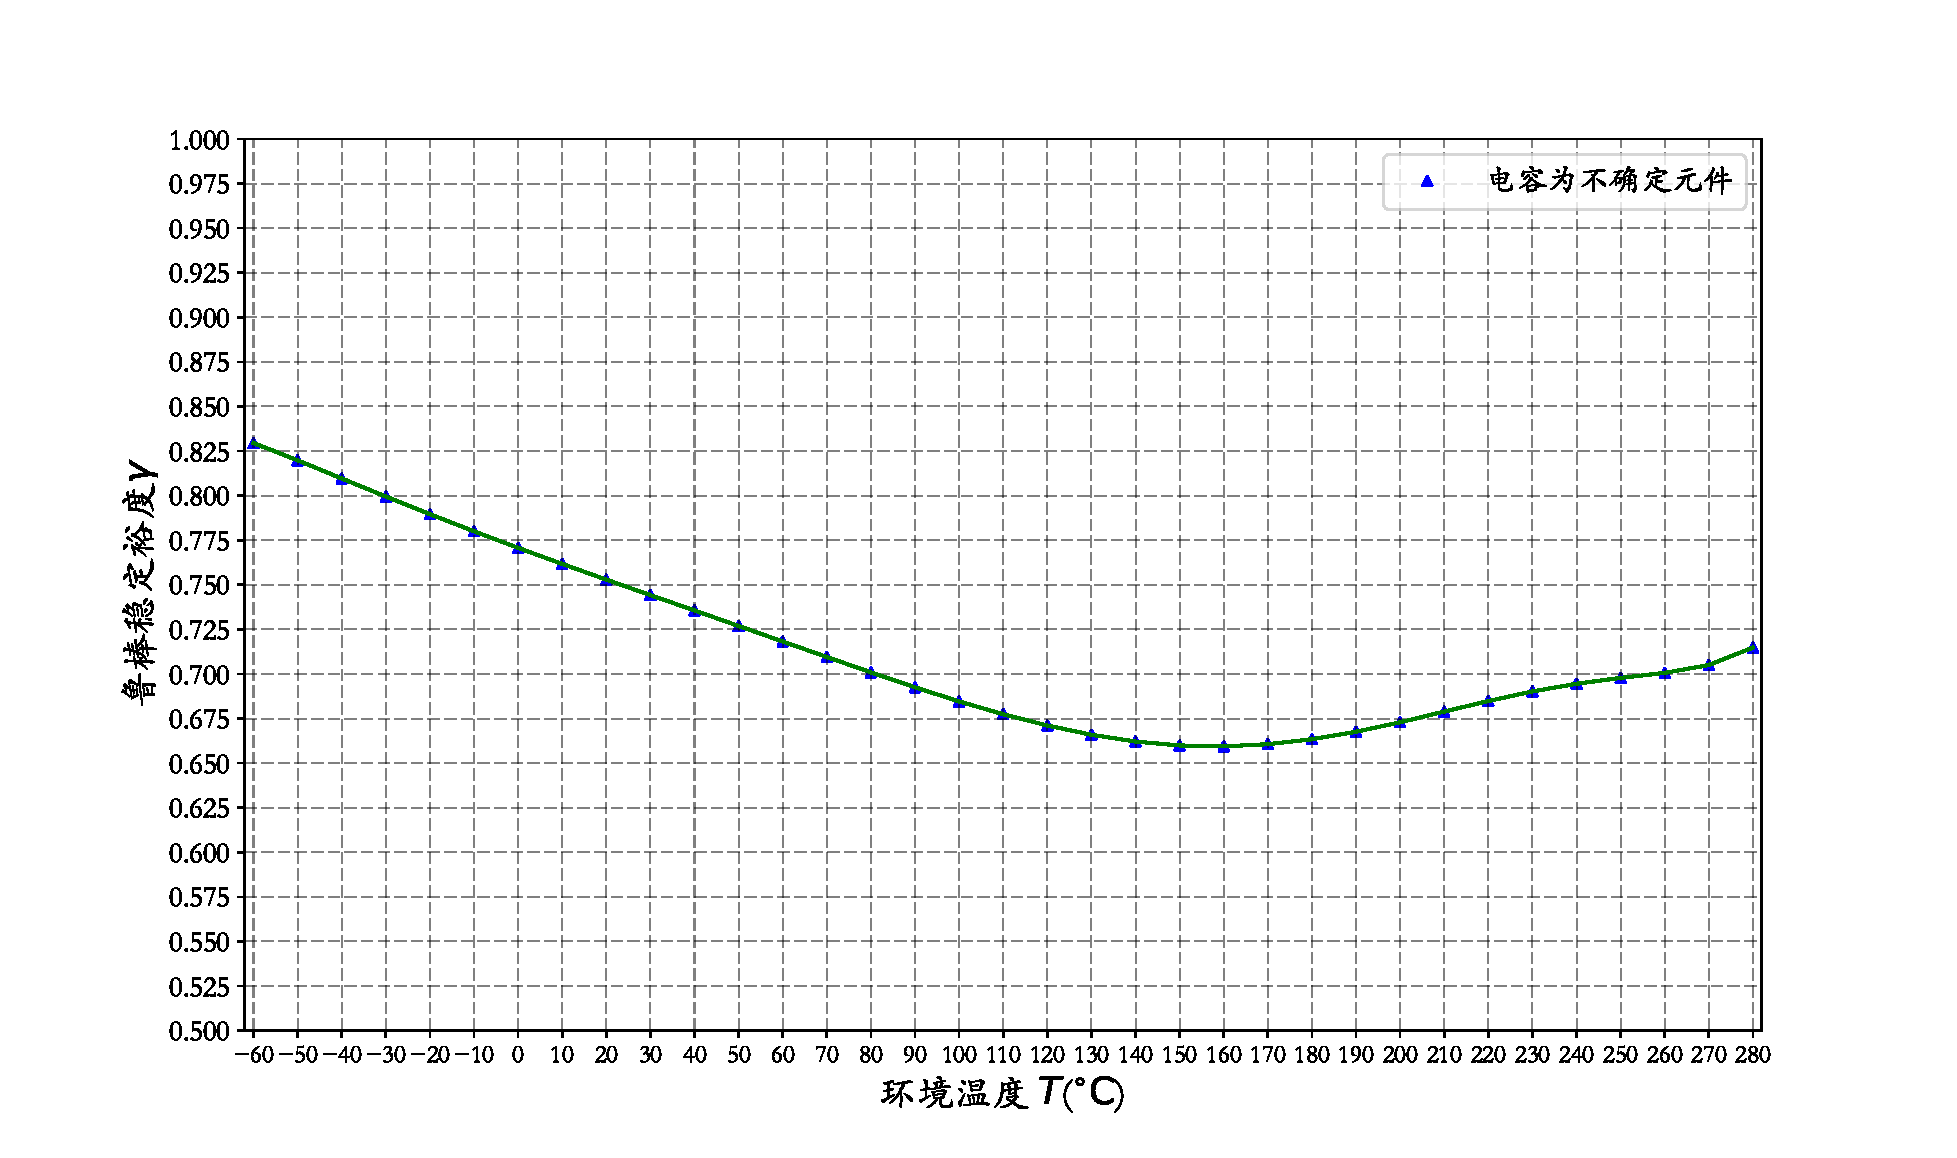
\includegraphics[width=14cm]{C_uncertainty.pdf}\\
      \medskip
  %\includegraphics[width=12cm]{test_speed_step.png}\\
  \caption{电容元件不确定时不同工作环境中系统鲁棒稳定裕度}\label{fig:chap5:cuncertainty}
\end{figure}

(2)~根据脆弱性指标的计算公式,求出未经归一化的脆弱性指标向量为~:
\begin{equation}\label{equ:chap5:Index30}
IND_0=\left[
\begin{matrix}
~~4.97\times10^{-4} &0.2842  &1.063\times10^{-3}  &1~~
\end{matrix}
\right]
\end{equation}

根据离差标准化处理后可得归一化的脆弱性指标向量为~:
\begin{equation}\label{equ:chap5:Index31}
IND=\left[
\begin{matrix}
~~0.1691  &0.2842  &0.0043  &0.1~~
\end{matrix}
\right]
\end{equation}

(3)~依据~4.4.2~节基于主观评价的指标权重分配方法,分配四个脆弱性量化指标的权重,可得权重分配向量为~:
\begin{equation}\label{equ:chap5:Index32}
W=\left[
\begin{matrix}
~~0.1570 &0.2720  &0.4829  &0.0882~~
\end{matrix}
\right]
\end{equation}

(4)~根据以上计算结果,可得基于~Buck~变换器的空间电源系统在电容不确定的情况下系统脆弱性的量化评估结果为~:
\begin{equation}\label{equ:chap5:Index33}
V_C=IND\cdot W^T=0.1147
\end{equation}
\subsection{电感元件不确定时系统脆弱性分析与量化评估}
基于~Buck~变换器的空间电源系统在电感元件不确定时系统脆弱性量化评估的具体过程包含以下步骤~:

(1)~对于电感元件不确定的情况,对~MATLAB~软件计算得到的系统鲁棒稳定裕度参数~$\gamma_L$~进行多项式拟合,拟合曲线如图~\ref{fig:chap5:luncertainty}~所示。得到电感不确定情况下,系统鲁棒稳定裕度参数~$\gamma_L$~随温度~T$\left(^{\circ}C\right)$~变化的函数表达式
\begin{equation}\label{equ:chap5:Index34}
\begin{split}
   \gamma_L= &3.866\times10^{-17}\cdot T^7-2.839\times10^{-14}\cdot T^6+6.517\times10^{-12}\cdot T^5-3.46\times10^{-10}\cdot T^4\\
     & -2.817\times10^{-8}\cdot T^3+2.525\times10^{-6}\cdot T^2-9.373\times10^{-4}\cdot T+0.7242
\end{split}
\end{equation}
\newpage
多项式拟合的参数指标为:

\qquad 误差平方和~$SSE\colon~~1.54\times10^{-5}$  \qquad 均方差~$MSE\colon~~4.40\times10^{-7} $

\qquad 均方根~$RMSE\colon~~~~6.63\times10^{-4}$    ~~\qquad 确定系数~$R-square\colon~~0.9998$

\iffalse
\begin{table}[htbp]
  \centering
\begin{tabular}{p{5cm}p{5cm}}

  误差平方和~$SSE\colon~~1.54\times10^{-5}$     &~~均方差~$MSE\colon~~4.40\times10^{-7} $\\

  均方根~$RMSE\colon~~6.63\times10^{-4}$        &~~确定系数~$R-square\colon~~0.9998$ \\
\end{tabular}
%  \caption{}\label{tab:chap5:canshu}
\end{table}
\fi
\begin{figure}[h]
  \centering
  % Requires \usepackage{graphicx}
     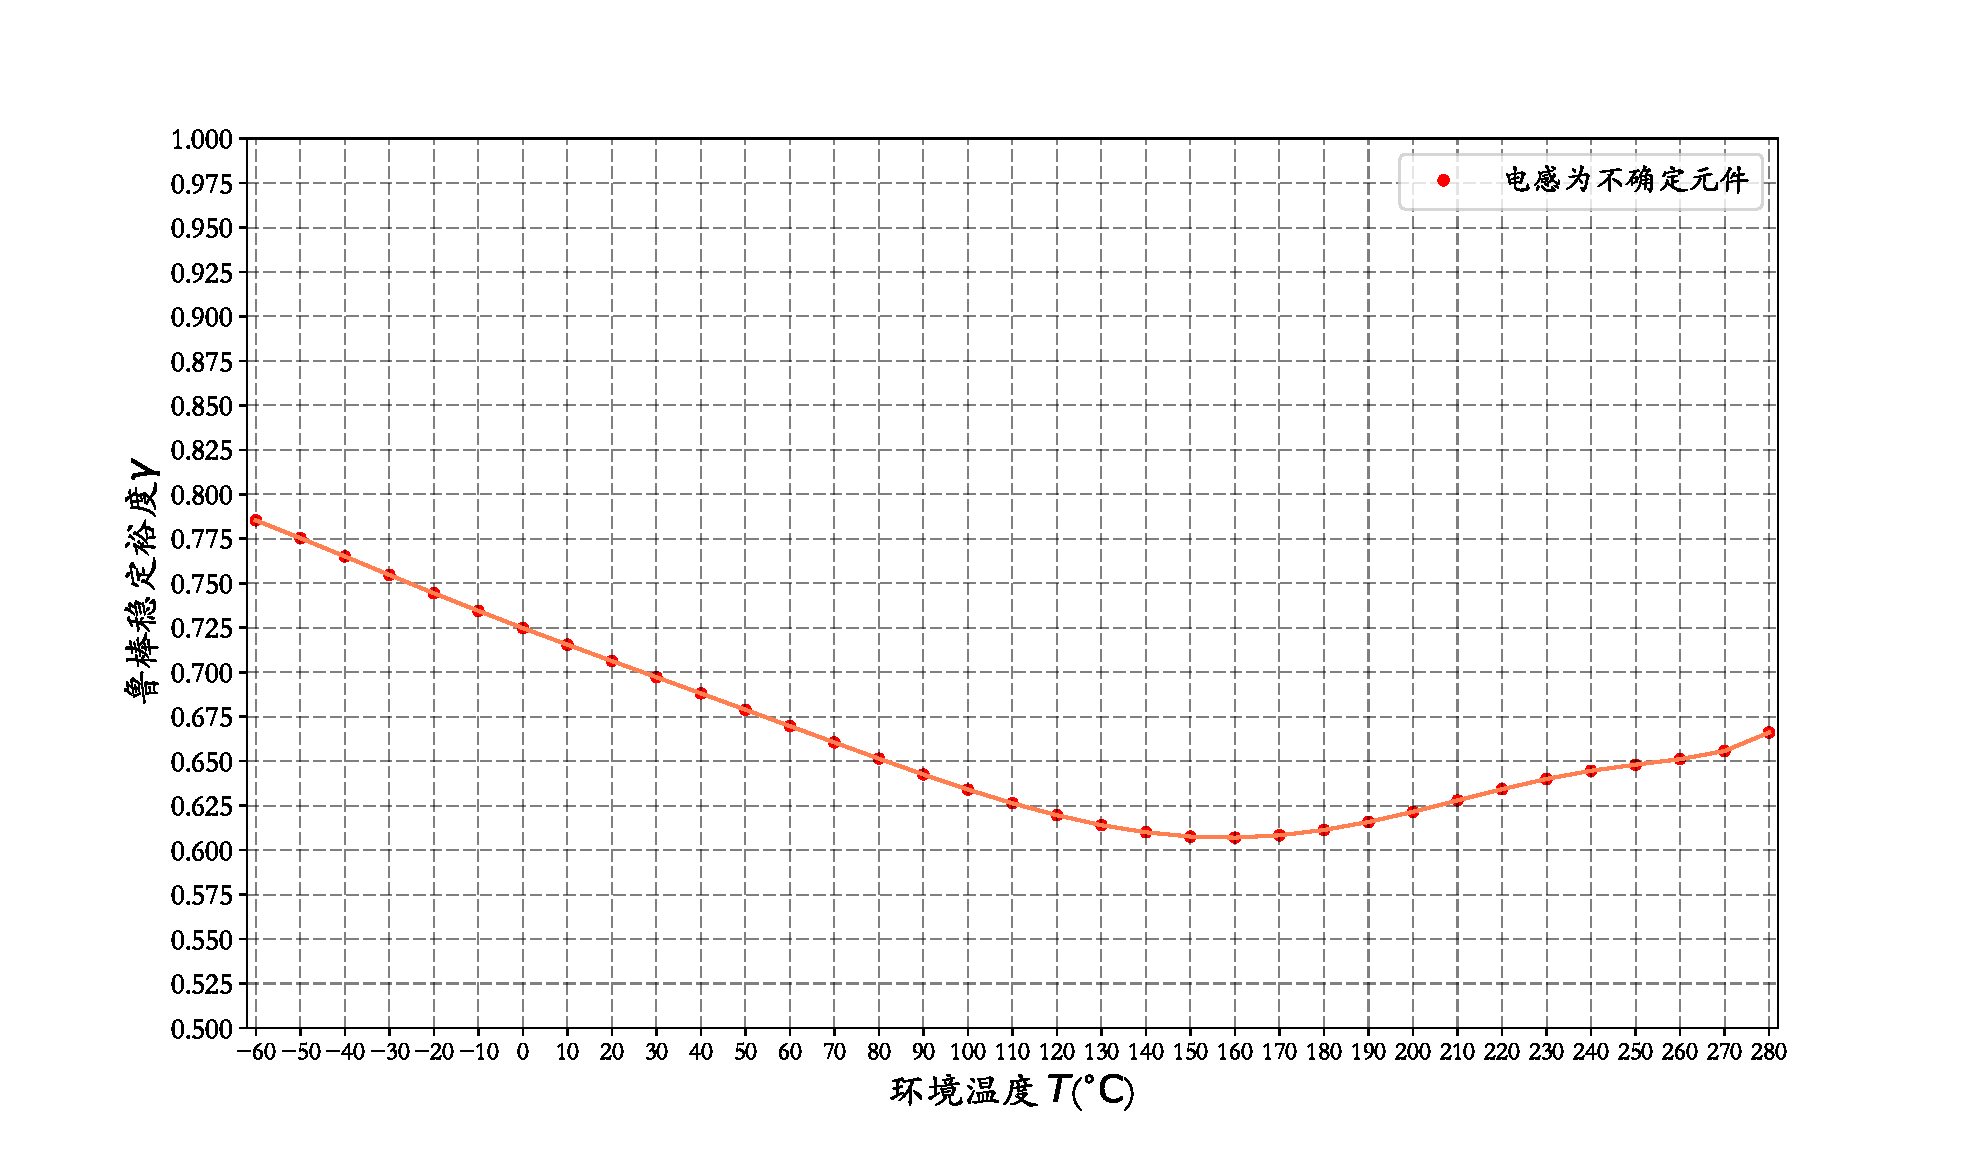
\includegraphics[width=14cm]{L_uncertainty.pdf}\\
     \medskip
  %\includegraphics[width=12cm]{test_speed_step.png}\\
  \caption{电感元件不确定时不同工作环境中系统鲁棒稳定裕度}\label{fig:chap5:luncertainty}
\end{figure}

(2)~根据脆弱性指标的计算公式,求出未经归一化的脆弱性指标向量为~:
\begin{equation}\label{equ:chap5:Index35}
IND_0=\left[
\begin{matrix}
~~5.21\times10^{-4} &0.3332  &1.097\times10^{-3}  &1~~
\end{matrix}
\right]
\end{equation}

根据离差标准化处理后可得归一化的脆弱性指标向量为~:
\begin{equation}\label{equ:chap5:Index36}
IND=\left[
\begin{matrix}
~~0.1771 &0.3332  &0.0044  &0.1~~
\end{matrix}
\right]
\end{equation}

(3)~依据~4.4.2~节基于主观评价的指标权重分配方法,分配四个脆弱性量化指标的权重,可得权重分配向量为~:
\begin{equation}\label{equ:chap5:Index37}
W=\left[
\begin{matrix}
~~0.1570 &0.2720  &0.4829  &0.0882~~
\end{matrix}
\right]
\end{equation}

(4)~根据以上计算结果,可得基于~Buck~变换器的空间电源系统在电感不确定的情况下系统脆弱性的量化评估结果为~:
\begin{equation}\label{equ:chap5:Index38}
V_L=IND\cdot W^T=0.1294
\end{equation}
\subsection{电阻元件不确定时系统脆弱性分析与量化评估}
基于~Buck~变换器的空间电源系统在电阻元件不确定时系统脆弱性量化评估的具体过程包含以下步骤~:

(1)~对于电阻元件不确定的情况,对~MATLAB~软件计算得到的系统鲁棒稳定裕度参数~$\gamma_R$~进行多项式拟合,拟合曲线如图~\ref{fig:chap5:runcertainty}~所示。得到电阻不确定情况下,系统鲁棒稳定裕度参数~$\gamma_R$~随温度~T$\left(^{\circ}C\right)$~变化的函数表达式
\begin{equation}\label{equ:chap5:Index39}
\begin{split}
   \gamma_R= &5.312\times10^{-20}\cdot T^7-3.509\times10^{-17}\cdot T^6+6.048\times10^{-15}\cdot T^5+3.155\times10^{-13}\cdot T^4\\
     & -1.642\times10^{-10}\cdot T^3+2.226\times10^{-8}\cdot T^2-3.47\times10^{-6}\cdot T+0.9008
\end{split}
\end{equation}

多项式拟合的参数指标为:

\qquad 误差平方和~$SSE\colon~~2.88\times10^{-12}$  \qquad 均方差~$MSE\colon~~8.23\times10^{-14} $

\qquad 均方根~$RMSE\colon~~~2.87\times10^{-7}$    ~~~~~\qquad 确定系数~$R-square\colon~~0.9999$

\iffalse
\begin{table}[htbp]
  \centering
\begin{tabular}{p{5cm}p{5cm}}

  误差平方和~$SSE\colon~~2.88\times10^{-12}$     &~~均方差~$MSE\colon~~8.23\times10^{-14} $\\

  均方根~$RMSE\colon~~2.87\times10^{-7}$           &~~确定系数~$R-square\colon~~0.9999$ \\
\end{tabular}
%  \caption{}\label{tab:chap5:canshu}
\end{table}
\fi
\begin{figure}[h]
  \centering
  % Requires \usepackage{graphicx}
     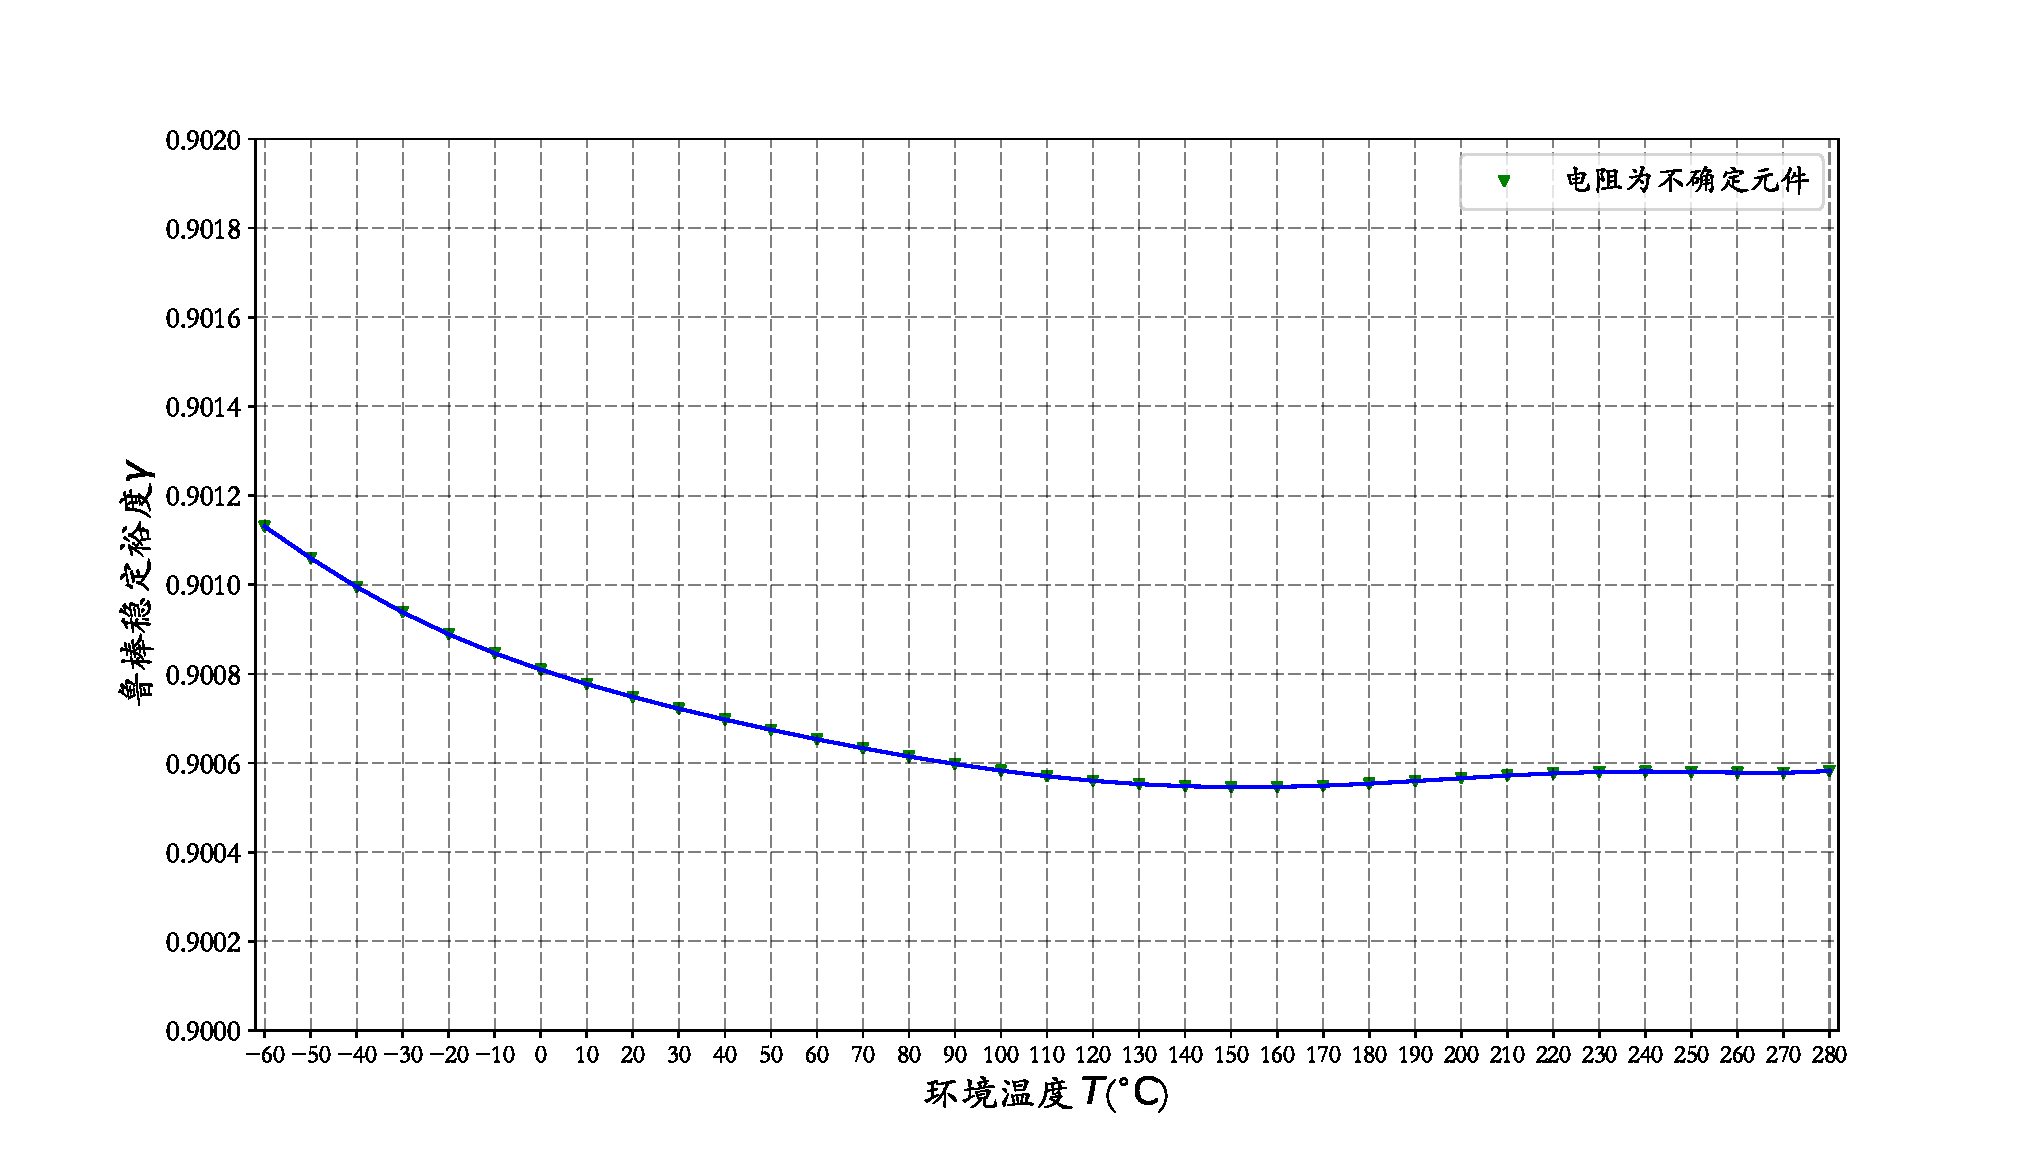
\includegraphics[width=14cm]{R_uncertainty.pdf}\\
     \medskip
  %\includegraphics[width=12cm]{test_speed_step.png}\\
  \caption{电阻元件不确定时不同工作环境中系统鲁棒稳定裕度}\label{fig:chap5:runcertainty}
\end{figure}

(2)~根据脆弱性指标的计算公式,求出未经归一化的脆弱性指标向量为~:
\begin{equation}\label{equ:chap5:Index35}
IND_0=\left[
\begin{matrix}
~~1.72\times10^{-6} &0.0993  &7.615\times10^{-3}  &3~~
\end{matrix}
\right]
\end{equation}

根据离差标准化处理后可得归一化的脆弱性指标向量为~:
\begin{equation}\label{equ:chap5:Index36}
IND=\left[
\begin{matrix}
~~0.0006 &0.0993  &3.0458\times10^{-5}   &0.3~~
\end{matrix}
\right]
\end{equation}

(3)~依据~4.4.2~节基于主观评价的指标权重分配方法,分配四个脆弱性量化指标的权重,可得权重分配向量为~:
\begin{equation}\label{equ:chap5:Index37}
W=\left[
\begin{matrix}
~~0.1570 &0.2720  &0.4829  &0.0882~~
\end{matrix}
\right]
\end{equation}

(4)~根据以上计算结果,可得基于~Buck~变换器的空间电源系统在电阻不确定的情况下系统脆弱性的量化评估结果为~:
\begin{equation}\label{equ:chap5:Index38}
V_R=IND\cdot W^T=0.0536
\end{equation}
\subsection{基于~Buck~变换器空间电源系统脆弱性综合分析}
根据空间电源系统电容、电感、电阻元件的脆弱性分析可知,在电容、电感以及电阻元件参数具有~$\pm10\%$~不确定性的情况下,脆弱性量化分析结果如表~\ref{tab:chap5:fragility}~所示。
\begin{table}[htbp]
  \centering  \caption{元件参数在~$\pm10\%$~不确定性时脆弱性量化评估结果}
  \label{tab:chap5:fragility}
\begin{tabular}{C{3cm}C{3cm}C{3cm}}
\toprule
  $V_C$         &$V_L$         &$V_R$\\
\midrule
  $0.1147$     &$0.1294$     &$0.0536$\\
\bottomrule
\end{tabular}
\end{table}

经过补偿环节的~Buck~变换器电源系统具有较好的系统性能,对于电容、电感以及电阻元件参数具有~$\pm10\%$~不确定的情况,系统脆弱性量化评估结果都比较小,即系统脆弱性分析结果良好。分别对比三种情况脆弱性量化评估结果可知,电源系统在电阻元件存在~$\pm10\%$~不确定时系统脆弱性量化评估结果~$V_R$~最小,即电阻元件不确定性对系统脆弱性影响较小。电源系统在电感元件存在~$\pm10\%$~不确定时系统脆弱性量化评估结果~$V_L$~最大,即电感元件不确定性对系统脆弱性影响较大,则电感元件为易导致系统脆弱性的薄弱环节。

在实际工程问题中,电子元件的不确定性是由特殊的工作情况与工作环境导致的。产生元件参数不确定性的原因林林总总,为避免对每一种情况都进行研究,分析与设计空间电源系统时可进行冗余分析,针对电源系统关键元件的最大不确定性进行最坏情况分析,得到最坏情况下系统脆弱性分析与量化评估结果,在空间电源系统电路设计与系统集成等方面具有现实意义。
\section{本章小结}
\label{sec:chap5:sum}
本章以基于~Buck~变换器的空间电源系统作为研究对象,采用本文建立的脆弱性分析方法与量化评估模型进行脆弱性分析,给出了脆弱性分析与量化评估的具体步骤。

依据前文对系统不确定性的分析,建立了基于~Buck~变换器的空间电源系统在电容元件、电感元件以及电阻元件存在不确定性情况下的系统模型。根据第二章建立的恶劣环境中电子元器件退化模型,模拟在不同工作环境中基于~Buck~变换器空间电源系统的工作状态。借助~MATLAB~软件平台,分析与计算在不同工作环境中空间电源系统的鲁棒稳定裕度参数。依据本文建立的脆弱性分析与量化评估数学模型,分别计算电容元件、电感元件以及电阻元件存在不确定性的系统在不同工作环境中的鲁棒稳定裕度参数,得到相应的脆弱性量化评估结果。

根据量化评估的结果,基于~Buck~变换器空间电源系统对于电子元件参数具有~$\pm10\%$~不确定的情况,经过参数补偿的电源系统具有良好的脆弱性指标,其中电感元件不确定性对系统脆弱性影响较大,电阻元件不确定性对系统脆弱性影响较小。在空间电源电路设计以及系统集成阶段,脆弱性分析方法与量化评估模型提供了一种分析与评估关键元件不确定性对系统脆弱性的影响程度的方法,对优化空间电源系统设计具有现实意义。